% Chapter 2

\chapter[Far-IR double-Fourier interferometers and their spectral sensitivity]{Far-infrared double-Fourier interferometers and their spectral sensitivity} % Main chapter title

\label{chap:phasenoisepaper} % For referencing the chapter elsewhere, use \ref{Chapter1} 

%----------------------------------------------------------------------------------------

\section{Introduction}
%Observations at mid- to far-infrared wavelengths from the Earth's surface are extremely 
%limited by the large atmospheric opacity in this region of the spectrum. Space-based telescopes 
%like IRAS \cite[12-100 $\um$;][]{1984ApJ...278L...1N}, ISO \cite[2.5-240 $\um$;][]{1996A&A...315L..27K}, \textit{Spitzer} \cite[3.6-160 $\um$;][]{2004ApJS..154....1W}, AKARI  \cite[1.7-180 $\um$;][]{2007PASJ...59S.369M}, WISE \cite[3.4-22 $\um$;][]{2010AJ....140.1868W} and \textit{Herschel} \cite[55-672 $\um$;][]{2010A&A...518L...1P} have demonstrated the scientific value of observations at 
%these wavelengths; but the spatial resolution of space-based observatories is limited by the cost 
%and complexity of building and flying progressively larger aperture telescopes. 
%Interferometry is a common solution to this problem on the ground, and is a viable path forward to obtain much
%higher resolution than what single apertures can provide. 
%In particular, spatio-spectral interferometry \citep{Mariotti:1988vea} is a way to achieve 
%high angular and spectral resolutions at far-IR wavelengths from above the atmosphere, without the cost and limitations of large single apertures. 

Several space-based interferometer concepts, the Far Infrared Interferometer \citep[FIRI;][]{2009ExA....23..245H}, the Space Infrared Interferometer Telescope
\citep[SPIRIT;][]{Leisawitz:2007if}, and the Submillimeter Probe of the Evolution of Cosmic Structure \citep[SPECS;][]{Harwit:2006hl}, have been proposed and use spatio-spectral interferometry to achieve the much needed angular resolution to 
study astronomical processes such as the birth of stars and planetary systems, the activity in 
galactic nuclei and the formation of galaxies in the distant universe. The FIRI and SPIRIT concepts have
two mirrors which are movable on one axis along a monolithic truss to provide a range of baseline lengths.
%the angle of the baselines is changed by rolling the spacecraft about the line of sight to the desired target. 
SPECS consists of three spacecraft connected via tether to achieve baselines of order 1~km. 

There are numerous engineering challenges to be addressed before such missions can become reality. A number of them can be tackled with testbeds \citep[e.g.][]{Leisawitz:2012ik, 2012ApOpt..51.2202G} and small-scale pathfinder missions. These missions 
will likely be two-element, single baseline interferometers in space or on balloon platforms,
such as the Balloon Experimental Twin Telescopes for Infrared Interferometry \cite[BETTII;][]{Rinehart:2014gk} and to a certain extent the Far-Infrared Interferometric Telescope Experiment \cite[FITE;][]{Kato:2010jf}.  
These pathfinders will have very limited baseline coverage and
rather than producing full images, they will focus on reconstructing 
spectral information from closely-spaced sources. This paper explores
aspects of the noise in spectral measurements specific to these instruments.

\subsection{Spatio-spectral interferometry}

In their pioneering paper, \citet{Mariotti:1988vea} lay out the principles of spatio-spectral 
(or double-Fourier) interferometry. A spatio-spectral interferometer consists of a Fourier transform 
spectrometer (FTS), where a delay line mechanism modulates the optical path difference (OPD) between two independent light beams before combining them in the pupil plane. The instrument produces interferograms, which are arrays of power measurements as a function of the OPD. Unlike traditional FTS, 
where a single incoming beam is split, delay-modulated, and recombined, a double-Fourier 
interferometer utilizes multiple light collectors pointing to the same astronomical source and 
combines the incoming light from the collectors pairwise in the pupil plane. The orientation 
and magnitude of the baselines - the vectors between each pair of light collectors - determines 
which  spatial frequency of the astronomical image the instrument measures. 
Longer baselines correspond to higher angular resolutions. The ``double-Fourier" aspect comes from 
the fact that the interferogram measured on a given baseline is related to the Fourier Transform (FT)
of the spatial and spectral distribution of the source emission.
Two FTs are used to reconstruct the full spatio-spectral datacube representing the 
astronomical scene: the spectra which are more directly related to the power as a function of time
delay difference between the two incoming beams (equivalent to the OPD) and
the source 2D spatial structure on the sky which is more directly related to measurements
accumulated from many different baseline vectors. The length of the baseline vectors can be changed by modifying the distance between the light collectors. The orientation of the vectors can be changed by rotating the baseline with respect to the source on the sky.
The plane representing the source visibilities
as a function of baseline vector is referred to as the ($u, v$)-plane and is a common notion in ground-based submillimeter and radio interferometry. This paper focuses on the reconstruction of the spectrum from closely-spaced point sources using single-baseline measurements, and does not address the techniques and sensitivities involved in using multiple baseline lengths to produce an image of the scene; a mathematical formalism that covers imaging is already proposed in \citet{Elias:2007jsa}.

%LGM: ZPD dependence within columm for large offset not done

Proposed double-Fourier instruments at far-IR wavelengths distinguish themselves from operating interferometers at sub-millimeter and radio wavelengths in several ways. First, they do not directly measure the phase information. The fundamental measurement is a time series of real-valued power as a delay line modulates the OPD in a controlled sequence (for example a linear ramp). The OPD from the delay line, as well as other OPD contributors in each arm of the instrument, and the external OPD created when the line of sight to a source is not perpendicular to the baseline vector, add up to the total OPD.
In double-Fourier instruments, the OPD can be determined by measuring or estimating the various contributors to the total OPD. For a given detector location along the projected baseline vector, there exists a value of the OPD in the delay line that exactly compensates all other OPD contributors. This delay line position results in a zero net total OPD, and is called the Zero Path Difference (ZPD). At this value of OPD, an incoming plane wave traverses the two beam paths reaching the detector exactly with the same phase, for all wavelengths. ZPD corresponds to the center of an interferogram for that detector location. In the
context of this paper, the phase for a given wavelength $
\phi_\lambda$ is related to the OPD between the beams from each arm when they combine, at the time of a data point measurement: $\phi_\lambda = 2\pi\textrm{OPD}/ \lambda$.
%LGM: rearraged above paragraph to define phase later and keep focus on path difference

% In the context of this paper, the "phase" refers to the total optical delay between the beams from both arms when they are combined, for a given location on the detector array. The total OPD is influenced by the OPD between the arms of the instrument, the OPD introduced by the delay line, and  In double-Fourier instruments, the phase for each point of the interferogram can only be known indirectly by measuring or estimating these three OPD contributors: while the measured signal is an power as a function of delay line OPD, the physical information lie in the measured power as a function of total OPD (or phase). For each detector location along the baseline vector, there exists a value of delay line OPD that will exactly compensate the other OPD contributors, hence making the net OPD zero. This point, called the Zero Path Difference (ZPD), is the center of an interferogram at that detector location. Hence, measuring the location of the center of an interferogram can be used to retrieve the phase for each of the points in the interferogram, provided that other factors stay constant

%It is possible, for example, to accurately estimate the phase for each point of the interferogram if the Phase information is derived from acquired knowledge of the true Zero Path Difference (ZPD, equal optical path length for a target position on the sky).

A second important difference for balloon and space interferometers is that collectors are not fixed
to the Earth. In the case of BETTII and SPIRIT, the collectors are fixed to a truss structure which
is part of the mechanical system for pointing the collectors. Consequently, baseline length
and external OPD, as relevant to an astronomical source, are not independent of pointing errors. The impact of errors in baseline length is modest because the relevant measure is in terms of fractions of the collector diameter. Errors in pointing translate into external OPD as the sine of the error angle times the baseline length, while the relevant measure is the wavelength. This can easily become significant;
for example, a 1" pointing error for an 8~m long baseline corresponds to a $38~\um$ shift in OPD.
%LGM: Added last sentence

\begin{figure}[ht!]
\begin{center}
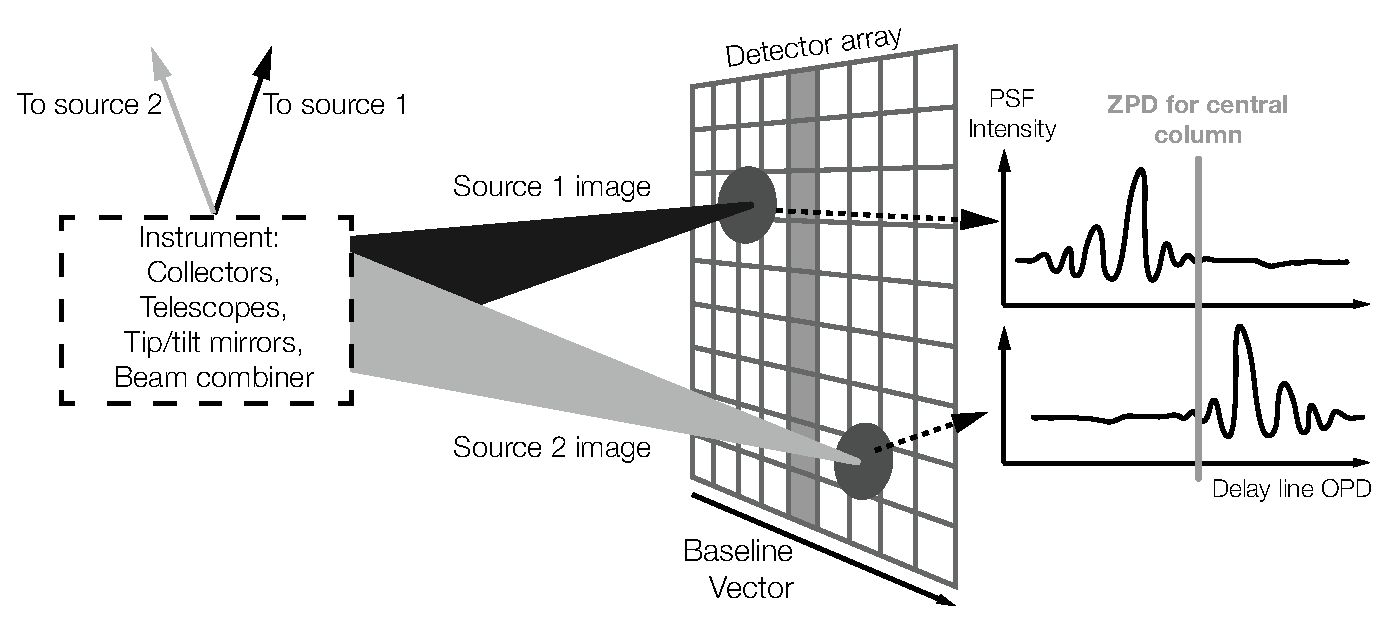
\includegraphics[width=\textwidth]{Figures/f1.eps}
\caption[WideField]{Concept of wide-field double-Fourier interferometry. Light from the instrument is focused after combination to an image of the sky on the detector array (represented as the grid). Each column of the detector has a distinct ZPD so the interferometric responses (right side) of two sources on different columns are centered around different delay positions. The gray stripe represents the central column on the detector array and its corresponding ZPD on the interferograms.}
%The instrument is represented by the double-headed arrow to the left. This encompasses the light collectors, the telescopes, the tip/tilt correction stages, the pupil re-imagers, and the beam combiner. After the beam combiner, the beam is focussed onto the detector array shown in this picture. Changing the OPD modulates the intensity of the Airy disks of each source in the field, and we get interferograms, as shown to the right. In this sketch we suppose that the baseline is aligned with the rows on the detector. Hence, each column of pixels always has the same instrumental OPD. In the general case, pixels along a line perpendicular to the baseline have the same OPD. Further, each source at an angle $\theta$ from the central column has an external OPD equal to $|\baseline |\sin\theta$. When the instrumental OPD approaches the opposite of this value, fringes can be seen for the source.}
\label{fig:widefield}
\end{center}
\end{figure}


Third, bolometer-type detectors, such as being built for BETTII and envisioned for SPIRIT, are
easily, and indeed typically, configured as two-dimensional arrays. With pupil plane combination,
the entire field of view has an interferometric response; hence wide-field interferometry over
multi-pixel arrays is straightforward. Fig.~\ref{fig:widefield} shows this concept and sketches the instrumental
response. For the configuration shown with the detector array columns aligned perpendicular
to the baseline vector, ZPD is the same along lines perpendicular to the baseline vector projected on the detector. As the OPD is swept, it moves across ZPD for the different columns in the array, yielding interferograms with shifted centers corresponding to the changes in external OPD for each source location in the field. 

By sweeping the OPD, the double-Fourier instrument measures interferograms which contain both spectral and spatial information over the detector array. The full spatial and spectral source information can be unambiguously recovered by repeating the delay line sweep over a range of baseline angles and lengths, which correspond to different spatial frequencies on the sky \citep{Mariotti:1988vea}.


\subsection{The case study: BETTII}

The BETTII project \citep{Rinehart:2014gk}, is a motivation for this paper and a near-term application of spatio-spectral interferometry. BETTII consists of two 50~cm siderostats on a fixed 8~m baseline, with a far-IR beam-combining instrument at the center. It will observe the far-IR universe in two 
wavelength bands, 30-50~$\um$ and 60-110~$\um$. The instrument is currently under construction at NASA Goddard Space Flight Center and is scheduled to launch in the Fall of 2016 on a stratospheric balloon from Fort Sumner, New Mexico, to an altitude of 35~km in order to be above most of the atmosphere. For its first flight, BETTII will focus on the study of dense star formation in nearby clusters. While a complete image reconstruction is not possible due to the static baseline length, BETTII will help resolve point source objects that are 0.5-1" apart in the short and long band, respectively, more than ten times the spatial resolution of \textit{Spitzer} at 24~$\um$ and six times the resolution of SOFIA at 37~$\um$.  Combined with a modest spectral resolution of $\R=10 - 50$, BETTII will measure the spectral energy distributions (SEDs) of clustered young stars to determine their evolutionary stage, locate the origin of the far-IR emission, and improve our understanding of how stars accrete their mass in these very dense regions of stellar birth \cite[e.g. see][and references therein]{2014prpl.conf..149T}. For resolved sources, the fixed baseline will not completely lift degeneracies between the spectral and spatial information; however detailed source modeling can put constraints on the distribution of the far-IR emission
\citep[e.g][]{Whitney:2013cw}.
%LGM: modified last sentence and added recent reference for modeling.

In this chapter, we study how various types of noise propagate to the derived spectrum in an
instrument like BETTII or SPIRIT. In section~2, we establish a mathematical formalism that can be used to represent interferograms. In section~3, we look at the dominant types of noise in the interferogram and define the relevant timescales associated with spatio-spectral interferometers. In section~4, we derive the spectral signal-to-noise ratio ($\SNR$). In section~5, we apply these results to the special case of BETTII to derive its point source spectral sensitivity.

\section{Mathematical formalism}
\label{sec:formalism}

\begin{figure}[ht!]
\begin{center}
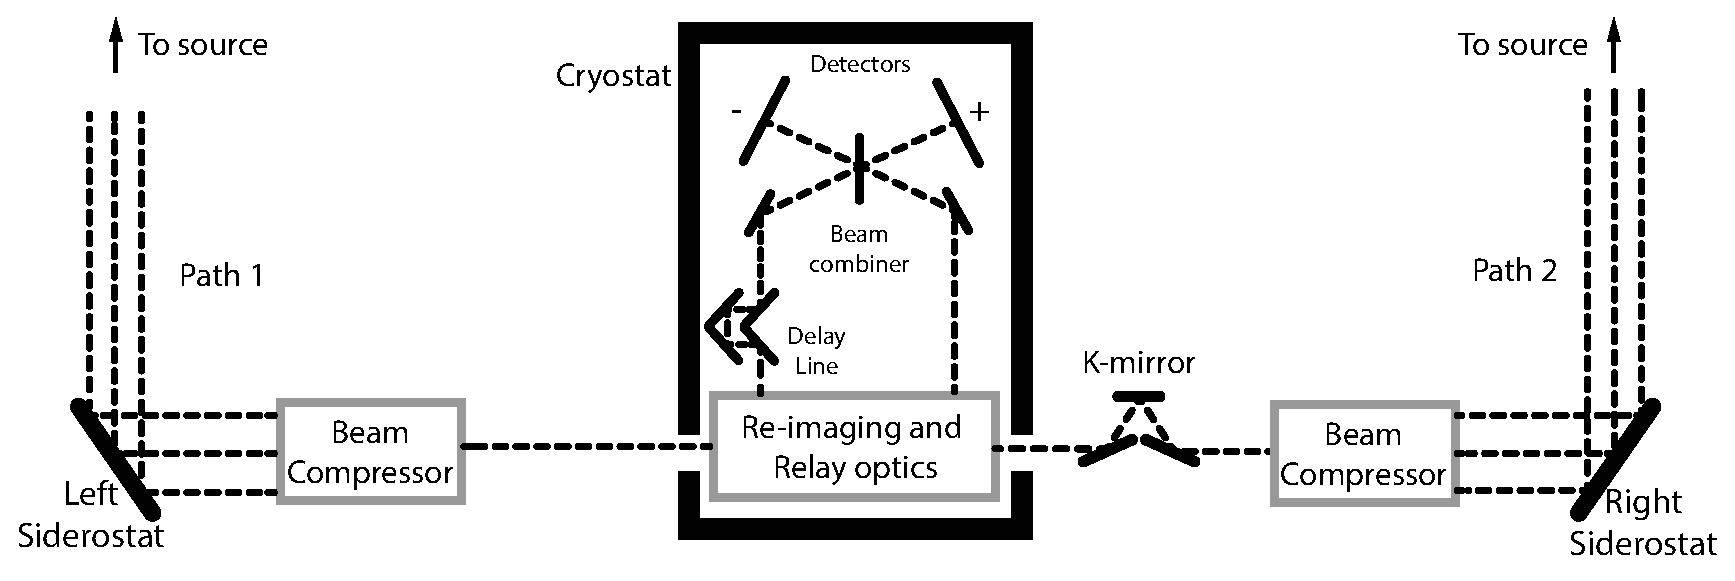
\includegraphics[width=\textwidth]{Figures/f2.eps}
\caption[Optics layout of Double-Fourier interferometers]{Optical train diagram of a typical far-IR, double-Fourier instrument. The K-mirror rotates the beam to align the fields of view of the two sides. Inside the cryostat, a set of optics re-image the pupil, implement a controlled instrumental delay between them with the Cold Delay Line, and relay them towards the central beam combiner. After the combiner, the beams are imaged onto the detectors. To see the BETTII-specific implementation of this design, see \citet{Rinehart:2014gk}.}
\label{fig:optics}
\end{center}
\end{figure}

The general optics layout for a double-Fourier system is shown in Fig.~\ref{fig:optics} for a single baseline. 
The combination of the siderostat and beam compressor acts as an afocal telescope 
which outputs a  parallel beam with a diameter convenient for the rest of the optical train.
The K-mirror in one beam path corrects for the pupil rotation so that the
images of the sky from the two collectors are matched over the field of view.
At the center of the instrument, there are optics for pupil re-imaging, filtering, and beam folding, as required by the specific implementation.
The key components for our purpose are the delay line, beam combiner and detectors. 
The delay line introduces a controlled OPD between both arms.
The two incoming beams are combined in the outputs from the beam combiner. 
We arbitrarily define one output as the ``+" and the other as the \mbox{``-"}. 
To conserve photon energy, the two outputs must be complimentary such that the summed power of the two is
independent of the OPD. In an ideal double-Fourier system, the two beam paths are symmetric about ZPD; 
hence, the power 
from the ``+" and ``-" outputs are equal at ZPD, and have odd symmetry about ZPD. In a traditional FTS at ZPD, one output has fully constructive interference while the other has fully destructive interference, with even symmetry about ZPD.

\subsection{Interferograms for a single baseline}

The interferogram for a single frequency of light measured at the outputs of the ideal double-Fourier instrument can be 
described in terms of the normalized intensity:
\begin{equation}
\hat{I}_\pm(x,\s) = \real(1 \pm i \; \Vb(\s) e^{-2i\pi \s x}),
\label{eq:basicinterferogram}
\end{equation}
where $\s \equiv {1 \over \lambda}$ is the wavenumber of the light in $\cm1$ as per the convention for the FTS literature, $x$ is the instrumental OPD created by the delay line with $x=0$ corresponding to ZPD, and $\Vb(\s)$ is the complex spatial visibility
%LGM: added x=0 statement above
 of the astronomical source for the baseline vector $\baseline$. ``$\real(f)$" indicates the real part of the complex-valued function $f$. The~$\pm$ indicates values for the two output beams: ``+" and ``-" in Fig.~\ref{fig:optics}.
%The "\textit{i}" in the second term of Equation 1 arises because the beam splitter puts a $\pi/2$ phase shift in the reflected beam.  The expression is the real part only because the measured interferogram is real valued. 
The derivation of this expression is given in Appendix~\ref{ap:interfero}.

The normalized complex spatial visibility $\Vb$ has a magnitude of 1 for all baselines for which the source is completely unresolved. For extended sources, the spatial visibility depends on the source geometry, intensity distribution, and the instrument baseline vector as described in Chapter~2 of \citep{Lawson:2000vf} 
and Chapter~3 of \cite{Thompson:2008ww}.  
For a normalized source brightness distribution $\hat{\F}$, the spatial visibility with respect to a phase reference position on the sky can be written as:
\begin{equation}
\Vb(\s)  =  \int_\textrm{source} d\Omega \Ahat(\Ds) \hat{\F}(\Ds ) e^{-2i\pi\s\Ds\cdot \baseline},
\label{eq:viseq}
\end{equation}
where $\Ahat$ is the normalized reception pattern of the collecting area; $\baseline$ is the baseline vector between the two collectors and $\Ds$ is the vector on the plane of the sky from the phase reference position to the infinitesimal solid angle $d\Omega$. The resulting visibility as a function of baseline vector is the 2-dimensional FT of the source's sky distribution. 
Since $\hat{\F}$ does not have to be symmetric with respect to the chosen phase center, $\Vb$ is in general complex and can be expressed as an amplitude and a phase, $\Phib(\s)$: $\Vb(\s)  =  |\Vb(\s)|e^{i\Phib(\s)} $.


%, where we are implicitly expressing that
%$\Phib$ is also a function of $\baseline$.

Real instruments have asymmetries, imperfections, and measurement errors which can create phase-shifts between the two optical paths and across the pupils.
% , and differences
%reflection, and transmission properties of optical elements in . 
Fixed instrumental effects 
can be represented by a normalized instrumental visibility loss term, 
$\Vi(\s)$ where the complex quantity $\Vi(\s) = |\Vi(\s)|e^{i\Phii(\s)}$, as described in details in Chapter~3 of \cite{2000plbs.conf.....L}, represents both amplitude losses and phase shifts (see Appendix~\ref{ap:interfero}). Additional phase errors can arise from
imperfect knowledge of the real-time optical path lengths which we will represent as
$e^{i\Phir(\s, x)}$, where $\Phir(\s, x)$ is the ``phase noise"; this term depends on the OPD $x$ through time-dependent phenomena such as mechanical jitters, temperature variations in
the optics support, or pointing errors. In the rest of this paper, we will mostly talk about this ``OPD noise", which is the physical source of the noise, whereas phase noise represents its effects on the interferogram.
The total complex visibility sampled at a single $\s$ by the system is $\Vb(\s)\Vi(\s) e^{i\Phir(\s, x)}$, and it is normalized such that, for an ideal instrument observing a point source, this quantity is equal to 1 at ZPD.

Using Eq. \ref{eq:basicinterferogram} for the monochromatic source, the polychromatic interferogram is the integral over $\s$ of this dimensionless response at each wavenumber. The total amount of power coming into the 2-aperture interferometer within a small wavenumber range $d\s$ is $2\Area \Bspec(\s) c d\s$ where $2\Area$ is the total aperture area in m$^2$, $\Bspec(\s)$ is the spectral flux density in W$\cdot$m$^{-2}\cdot$Hz$^{-1}$ and $c$ is the speed of light in cm$\cdot$s$^{-1}$. 
%LGM: The wavenumber $\s$ has units of cm$^{-1}$ to follow the convention in the FTS literature.
%LGM: added this to the  definition of wavenumbers after Eq 1  
Filters and optics in an instrument cause a wavenumber-dependent transmission profile $\Tbp(\s)$. The quantum efficiency of the detector can depend on wavenumber, $\etaD(\s)$. For multi-pixel detectors the interferogram is measured by matched filtering a point-spread function on a pixel array, which has some efficiency $\etamf$.% Optical elements such as filters and beam splitters/combiners can cause $\s$-dependent phase shifts. 

%Since optical elements along the two light paths are not perfectly
%identical, the source flux density, as seen at the detector, is modified by an instrument transmission function which
%can be complex:
%\begin{equation}
%T_{\inst}(\s) \equiv \etamf\etaD\Tbp \Vi = |T_{\inst}(\s)|e^{i\Phi_{\inst}(\s)},
%\end{equation}
%where all of the terms can be functions of $\s$.

The actual power measured by the instrument can be represented as:
%I_\pm(x) = \real\left(\A \int_0^{+\infty} T_{\inst} \B \left(1\pm i\; \Vb e^{i\Phir(\s, x)} e^{-2i\pi \s x}\right)cd\s \right),
\begin{equation}
I_\pm(x) = \Area c\int_0^{+\infty} \etamf\etaD\Tbp \Bspec \times
 \quad  \real \left[\left(1\pm i \Vi\Vb e^{i\Phir} e^{-2i\pi \s x}\right) \right]d\s,
\end{equation}
where the factor of 2 for the two apertures is dropped because it is implicit in Eq. \ref{eq:basicinterferogram}. All quantities within the integral can be functions of wavenumber, and all the instrumental phase and interferometric loss terms are in $\Vi$ and $e^{i\Phir}$.

Instead of considering each separate output, we use $\I = \I_+ - \I_-$ as our interferogram expression, which cancels out the constant term. We also introduce an interferometric instrument transmission function, which can be complex, which represents the normalized amplitude and phase of the interferogram for a point source of uniform spectrum and no phase noise:
\begin{equation}
T_{\inst}(\s) \equiv \Area c\etamf\etaD\Tbp \Vi = |T_{\inst}(\s)|e^{i\Phi_{\inst}(\s)},
\end{equation}

 We can then write the modulated signal as:
%I(x) = \real\left( 2 \A\int_{0}^{+\infty} i |T_{\inst}| \B \Vb e^{i\Phir(\s, x) + i\Phi_{\inst}(\s)} e^{-2i\pi \s x}cd\s \right).
\begin{equation}
I(x) = \real\left( 2\int_{0}^{+\infty} i |T_{\inst}| \Bspec \Vb e^{i\Phir + i\Phi_{\inst}} e^{-2i\pi \s x}d\s \right),
\label{eq:modsignal}
\end{equation}
where $\Bspec$ is real and $\Vb$ can be complex.

Eq.~\ref{eq:modsignal} can be turned into a Fourier transform by mirroring all quantities to negative wavenumbers. This
convention is explained in detail in \citet{Davis:2001tr} for FTS instruments; the odd symmetry of the interferogram for a system with one beam combiner
and the complex instrumental transfer function means that the incident spectrum on the detectors
must be mirrored to -$\s$ as the negative of the complex conjugate of +$\s$: 
$\S_e(\s) \equiv [T_{\inst} \Bspec \Vb]_e(\s) = {1 \over 2}\left[T_{\inst}(\s) \Bspec(\s) \Vb(\s) - T^*_{\inst}(-\s) \Bspec(-\s) \Vb^*(-\s)\right]$. 
We use the subscript $e$ to denote the reflected function, and will apply this convention in the rest of this paper; this reflection ensures that the integrals keep the same value when are expressed from $-\infty$ to $+\infty$, and does not affect the $\SNR$ estimates: although the signal appears to be divided by a factor of two, so is the noise, as it is spread between positive and negative frequencies.
The interferogram expression is then:
%\begin{equation}
%I(x) = \real\left( 2 \A\int_{-\infty}^{+\infty} i [T_{\inst} \B \Vb]_e  e^{-2i\pi \s x + i\Phir(\s, x)} c d\s \right).
%\end{equation}
\begin{equation}
I(x) = \real\left( \int_{-\infty}^{+\infty} i \S_e  e^{-2i\pi \s x + i\Phir} d\s \right).%\end{equation}
\label{eq:interfero2}
\end{equation}
%[CHANGE THIS TO: INCLUDE THE SINC FUNCTION WITHIN THE INTEGRAL AND DIVIDE IT UP LATER IN THE BANDPASS PROFILE]
\subsection{Measured interferograms}

In practice, the interferogram data are discrete measurements of a real-valued signal on the detectors. Like for most FTS instruments, each data point on the interferogram corresponds to an integration of the detector while the delay line is continually in motion. This decreases the amplitude of the interferogram due to the local smearing of the fringes, but it can be kept to low values by increasing the fringe sampling.
% For example, for constant delay line velocity $v$, a delay distance $\Dx=v\Dt$ is swept during an integration time $\Dt$. 
At each delay $\xn$, the interferogram has a measured value $\Ixn = \frac{1}{\Dx}\int_{\xn-\Dx/2}^{\xn+\Dx/2}\I(x)dx$. To first order, this has the effect of multiplying the power at each wavenumber by $\sinc(\pi\s\Dx)$. For the purpose of this paper, we consider this term to be included as part of the instrumental transmission $T_{\inst}$. Note that the value of the optical delay $\xn$ is the path difference from ZPD, not the physical location of the delay line, since there could be a multiplying factor between the two due to beam folding (e.g., for BETTII, a motion of 1~mm of the delay line creates 4~mm of OPD).
%LGM: Added "the path difference from ZPD" above
%The final, real-valued interferogram can be represented as:
%\begin{equation}
%\Ixn = Real(\A\times \intinf \eta \Tbp\Be\left|\Vb\Vi\right|\sin(2\pi\s\xn + \Phi)d\s,
%\label{eq:finvis}
%\end{equation}
%where $\Phi = \Phib+\Phii+\Phir$ is the sum of the phases corresponding to the source visibility, instrumental, and phase-delay  terms. The measured quantity $\Ixn$ has units of power. 

%\subsection{Fourier transform spectroscopy}
%\label{sec:FTS}

%For a source that is spatially unresolved for all wavenumbers in the bandpass ($\Vb(\s)=1$), the true source spectrum $\Be$ is recovered by Fourier transform of the interferogram with respect to the delay $x$. This is mathematically valid since we made the spectrum of the source symmetric using $\Be$ instead of $\B$, as described in \cite{Davis:2001tr}; this allows us to transform back and forth between the interferogram and the spectrum.

A discrete Fourier transform (DFT) is used to transform a discrete interferogram of $N$ measurements into a complex discrete spectrum with $N$ points. The resolving power of the instrument, $\R = \lambda / \D \lambda$, is dependent on the physical length scanned by the delay line $L$: $\R = L \s / 2 $ for a scan with symmetric length on both sides of ZPD. For these instruments where we scan through the whole interferogram, the data should be
sampled at least at the Nyquist rate for the interferogram response frequency of $\Dx = \lambda/2$. For a sampling exactly equal to Nyquist, we have the relationship: $N = 4 \R$.

For a double-Fourier instrument, as shown in Fig.~\ref{fig:widefield}, the ZPD for different columns on the array occurs at different delay positions $x_{\col}$, related to
the projected baseline length. The simplest way to express this is in terms of the angular offset on the sky of each column, $\xi$, along the
direction of the baseline, $\baseline$:
\begin{equation}
x_{\col} = | \baseline | \sin\xi \approx | \baseline | \xi = 48.7 \um \left({| \baseline | \over 10~\textrm{m}}\right) \ \left( {\xi \over 1~\textrm{arcsec}}\right) ,
\label{eq:delay}
\end{equation}
where we have filled in
practical units for an infrared instrument. For a far-IR interferometer working at $50~\um$, with
1-2~m diameter collectors, the delay shift across the collector point spread function (collector angular resolution) is several to ten wavelengths.
%LGM: Added PSF above to clarify the this is refering to the resolution of the collector
Hence the scan length to cover a wide-field array detector is comparable to the scan length required to achieve
$\R$'s of 100's to 1000's. This property is an important consideration for observation and data analysis strategies.
%With $x_0 = 0$ defined as the center of the interferogram, we can write:
%\begin{equation}
%\DFT(\Ixn) =\sum_{n=-N/2}^{N/2-1}\Ixn e^{2i\pi n k/N}.
%\end{equation}

The ideal interferogram for a point source from a perfect instrument is an odd function of the OPD $x$, so its DFT is purely imaginary. The noise in the interferogram will be converted into spectral noise in both the real and imaginary axes so the real axis is a proportional measure of the noise. 
Referring back to Eq.~\ref{eq:interfero2}, phase shifts caused by the instrumental transfer function and source spatial visibility will
break the anti-symmetry; in practice, the DFT of a measured interferogram is complex and the real and imaginary parts are of interest.
The scientifically interesting quantities are the source spectrum and source spatial visibility: $\B$ and $\Vb$; the fixed
instrumental terms have to be calibrated or properly modeled
by observing a bright point source of known spectrum. The techniques for calibrating FTS systems are well developed
\citep[e.g.][]{Davis:2001tr}, and there are many methods proposed to correct some phase and amplitude errors \citep[e.g.][]{Forman:1966wx, Sromovsky:2003in}. 

\begin{figure}[!h]
\begin{center}
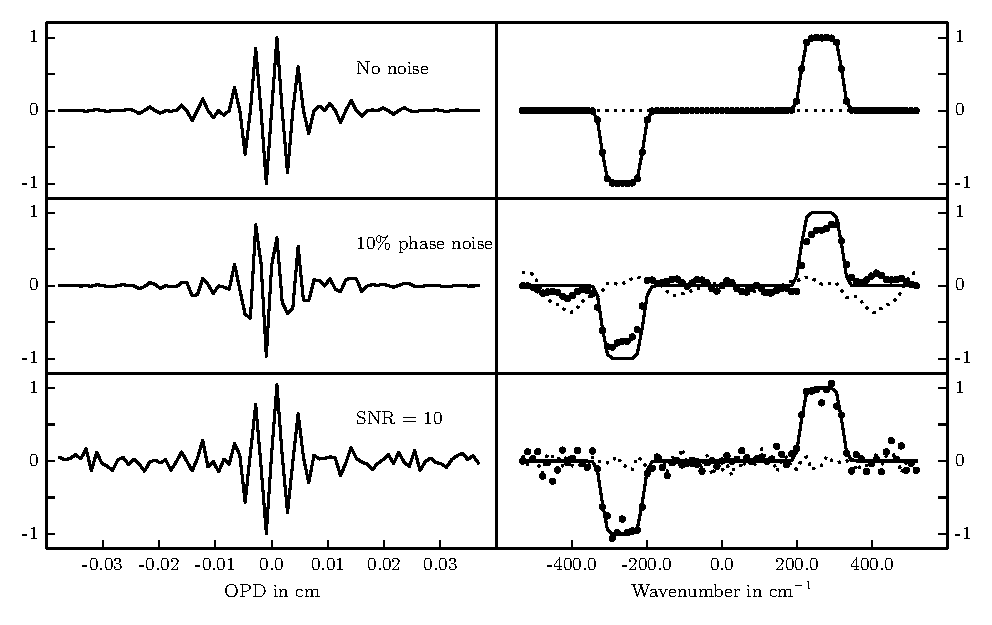
\includegraphics[width=\textwidth]{Figures/f3.eps}
\caption[interfero]{Effects of phase and intensity noise on the recovered spectrum (single realization of the noise). Left column: normalized interferograms, intensity as function of OPD. Right column: normalized DFT of interferograms. Solid: input spectrum multiplied by anti-symmetric transmission function; Solid circles: Imaginary part of DFT from interferogram; Dotted: Real part of DFT. First row: ideal measured signal, no noise; used for normalization of all other plots. Second row: results with a realization of phase noise of 10\% at each point of the interferogram. Third row: results with a realization of intensity noise and $\SNR_\mI=10$.}
\label{fig:interfero}
\end{center}
\end{figure}


The phase noise term $\Phir(x,\s)$ in Eq.~\ref{eq:interfero2}, and the $\SNR$ in the measured interferogram can have significant
impact on the ability to recover the source spectrum with a real instrument. The upper panel in Fig.~\ref{fig:interfero} shows an example of an interferogram (left), and the transformed $\S_e(\s_k)$ (right) for a source with flat power spectrum, multiplied by a flat bandpass function with smoothed edges.
 The middle panel of Fig.~\ref{fig:interfero} shows
the same source and instrument parameters as the upper panel, now with an assumed Gaussian OPD noise of standard deviation equal to 10\% of the central wavelength of the band $\lambda_0\equiv {1\over\s_0}$ (\textit{i.e.}, there is a $\lambda_0/10$ OPD uncertainty for each data point in the interferogram). The lower panel is the top panel observed with a incoherent background noise corresponding to $\SNR=10$ at the peak of the interferogram, and no phase noise. 
The next sections of this paper will analyze these noise contributions and quantify their impact on the derived spectrum.

\section{Noise sources}
The two primary types of noise in a double-Fourier instrument are intensity and OPD noise. The intensity
noise consists of the astronomical and thermal background noise, the photon noise from the source, and the detector noise. The OPD noise arises primarily from uncertainties and changes in OPD, which would prevent us from accurately knowing the $x$-values of measurements in the interferogram before the FT. For convenience, we usually refer to the OPD noise as a percentage of the carrier wavelength. In the rest of this paper, a ``10\% OPD noise" signifies that the OPD for each measurement in the interferogram is known to within an error of 10\% of the carrier wavelength, or 10\% of one full fringe cycle.

\subsection{Intensity noise}
\label{sec:noisesource}
The measured signal has units of power and can be represented as the interferometric signal with additive noise:
\begin{equation}
\Im\pxn = \Ixn + \ni\pxn,
\label{eq:thermalnoise}
\end{equation}
with $\ni$ being the difference of the noise in the two outputs of the interferometer, $\ni = \nA-\nB$. When the beam combiner, optical train, and detectors are symmetric, the residual $\ni$ has zero mean. 
The total noise in $\Im\pxn$, expressed in Noise Equivalent Power, $\NEPtot$, is the sum of the three noise variances: 
\begin{equation}
\NEPtot^2 = 2\NEPph^2 +2\NEPdet^2 +  2\NEPsou^2,
\end{equation}
where $\NEPph$ and $\NEPsou$ are the thermal noise from the background (e.g. sky and warm optics in the case of a far-IR instrument)
and source photon noise, respectively, in one output, and $\NEPdet$ is the noise-equivalent power characterizing each detector's noise (including phonon, readout and Johnson noise). The factor of 2 multiplies each term since we are considering the difference of both outputs.
The relation between $\NEPtot$ and the variance $\varI$ of the noise $\ni$ during an interval $\Dt$ is \citep{Sromovsky:2003in}:
\begin{equation}
\label{eq:sigI}
\varI = \frac{\NEPtot^2}{2\Dt}.
\end{equation}
For space instruments, the noise will likely be dominated by the sky background (zodiacal light, galactic cirrus emission, or optics thermal emission) and detector for a very large fraction of astronomical targets, which tend to be faint; for balloon instruments, emission from
warm optics and the atmosphere sets the noise level in the far-IR.

%There are three dominant sources of thermal photons at balloon float altitude for BETTII: the atmosphere, the dewar window, and the external optics (or telescope). Additional sources, such as the radiation coming from the Cosmic Microwave Background and the zodiacal disk, are much less significant at our observing wavelengths: our estimates show a five orders of magnitude difference. Hence, we will focus on the three main components when working out the noise budget of our instrument. The results are shown in Table \ref{tab:noise}. The values in the table correspond to the background levels per pixel. The sky radiance at float in our bands is taken from \citet{Harries:1980cva}. The radiance from the window and telescope assumes that they are blackbodies at 240~K, with respective emissivities of 0.02 and 0.08. The total optical efficiency assumed for the telescope is 30\%. Combining all these noise sources leads to a background NEP of $1.4\times 10^{-15}$ W.Hz$^{-0.5}$ in band 1 and $6.4\times 10^{-16}$ W.Hz$^{-0.5}$ in band 2. The detector NEP is expected to be less than $3\times 10^{-16}$ W.Hz$^{-0.5}$ in band 1 and $3\times 10^{-16}$ W.Hz$^{-0.5}$ in band 2.

\subsection{OPD noise}
\label{subsec:phnoise}
Observing from the ground at optical wavelengths with a double-Fourier interferometer is limited by the phase coherence 
between the apertures, which is related to the atmospheric coherence time, as discussed by \cite{Mariotti:1988vea}. The short coherence time forces fast scan rates, which degrades the sensitivity of the instrument due to short integration times and phase shifts between sequential scans. 
This is not a problem for flying platforms, since even at balloon altitudes the atmospheric coherence is not a significant 
issue \citep{Rizzo:2012jp}. The major concerns for balloon and space missions are overall instrumental stability, knowledge of ZPD, and pointing errors, which can all contribute to OPD noise.

OPD noise arises in an interferogram when the OPD at the time of a measurement is uncertain, hence compromising the reconstruction of the true $x$-value. Since this uncertainty is a physical delay $\delta_x$, 
the error in phase is wavenumber dependent: $2\pi\delta_x\s$. $\delta_x$ is the difference between the estimated $x$
and the true $x$.
% LGM: Added the sentence above.
% LGM I deleted the "_k$ on the wavenumber because this is not a discrete spectrum statement.
For single-beam FTS instruments, internal laser metrology can provide optical path length 
measurements to high accuracy \citep[e.g.][]{Griffiths:2007uu}, and the separate paths the split beams need to travel can be kept small. 
For double-Fourier instruments, the entire optical paths upstream of the beam combiner affect the OPD, hence it is more challenging to accurately measure and estimate the OPD contributors. 
In addition, common-mode pointing errors of the collectors are directly converted to geometrical delay errors. 
Hence, it is critical to know the position and orientation of the baseline vector with respect to the 
astronomical target with high accuracy in order to properly reconstruct the interferogram.

For this analysis, we identify three timescales that can be used to examine the effects of OPD noise on the interferogram. These timescales are important to consider in the design of the OPD control system of any double-Fourier interferometer. Timescale~1 is the shortest and corresponds to the integration time for a single data point, typically a few milliseconds. In practice, this kind of OPD noise could be created by high-frequency mechanical jitters in the instrument (including the delay line bearing and motor, stiction behaviors and resonant modes, reaction wheels and other self-induced vibrations...). Timescale~2 is the time it takes to acquire one single interferogram over the full field of view and at the desired resolving power, typically on the order of seconds. The sources of noise that can affect this timescale include for example pointing errors and drifts, as well errors in the knowledge of the delay line position relative to
a reference ZPD. Finally, the longest timescale to be considered, timescale~3, is the time it takes to complete one full "track" by co-adding several consecutive interferograms to achieve the desired $\SNR$, typically a few minutes long. During this timescale, it is expected that the change in baseline orientation on the sky does not produce any significant change in the source spatial visibility function. The latter timescale is most importantly influenced by thermal variations and time-varying gradients that could change the optical alignment and mechanical configuration between the two arms. 


%[It is important to realize that while the phase noise can be large during the data acquisition, some can be largely reduced in processing of the data with good models of the noise sources. With this in mind, the following noise derivations apply more on the residual uncertainties on a post-processed data product, rather than in-flight noise control. (PUT THIS SOMEWHERE ELSE?)]

%\subsection{Other sources of noise}

%Talk here about all other sources of noise? What are they actually?

%Our instrument has three relevant timescales for phase noise: 1) the integration time for a single data point (2 to 10~ms), 2) the time that it takes to gather one interferogram ($1-10$~s), and 3) the time over which $M$ interferograms are gathered to complete an observation ($\sim$~10~min). These timescales correspond to high frequency vibrations in the structure, pendulation motion of the instrument package hanging under the balloon, and a combination of pendulation, vertical "bobbing" motion of the balloon, and thermal changes, respectively. BETTII is designed and instrumented to mitigate the amplitude of these effects, but there will be residuals. 

%The interferometric delay $\delaytot$ of an astronomical source consists in the sum of the delays created by the position of the baseline with respect to the source, $\delayext$, and the delays that are internal to the instrument, $\delayint$. External delays change with the pendulum motion of the payload (intermediate timescale), while internal delays will change due to vibrations (short timescale) and thermal variations (long timescale). 

%The magnitude and frequencies of the perturbations for each timescale are difficult to estimate in detail. However, we will make some reasonable assumptions in order to predict sensitivities in the following sections. For the short timescale, the truss and support structure are designed to have lowest vibration modes above 20~Hz where dissipation in the structure will strongly damp oscillations. We expect the phase perturbations to be small over the 1-10~ms timescale. 

%The pendulum modes have been measured before on multiple experiments \cite[e.g.][]{Fixsen:1996kha} and have periods from 2 to 30 seconds and amplitudes up to 10~arcminutes. The highest frequency modes damp faster, especially for an experiment like BETTII that will be staring at inertial targets and not scanning the sky. The gondola pointing control system will compensate for most of these perturbations; we expect to be able to keep the gondola pointed at a given target to within 10-15 arcseconds, once the most powerful modes have damped. The pointing control system is described in detail in \cite{Rizzo:spie2014a}. The residual pointing errors of the gondola will result in external delay errors, and we can expect these errors to be generated at the same frequencies as the perturbations. BETTII will utilize
%measurements from the star camera, the fiber optics gyroscopes, and the tip-tilt pointing corrections to determine these residual errors with an expected accuracy of 1 arcsecond during flight. 
%MAXIME --- IS 1 arcsecond correct??? Put in the correct number.

%A second source of phase error in the intermediate timescale is self-created perturbations in the control loops for the pointing system and the delay lines. These perturbations can be minimized with optimal setting of the gain and bandwidth of the control loops. Post-flight knowledge of the pointing is expected to be accurate to $\sim$0.1~arcsec over a few minutes, and can be held longer when fringes are seen. Knowledge of the error in the commanded position of the delay stages will be measured in real time on BETTII with an accuracy of 0.2~$\um$ with capacitive sensors.

%Finally, thermal distortions are the most difficult to predict. They will depend on the radiative environment during ascent and at float, which is very hard to reproduce in a test environment without using a large vacuum chamber. We expect that the payload will be thermally stable on the order of 10~minutes but it is expected to be systematically cooling throughout most of the flight. 

%The pendulum modes can be very well estimated since they are much slower than any of our sensors (periods of 2~s minimum). Internal vibrations are hard to predict at this point, but they will be predictable we will be able to mitigate them on the ground. Further, they should be minimized by the good symmetry of the payload and our constant effort for synchronous control and command. Finally, thermal distortions are extremely hard to predict. They will depend on the radiative environment at float, which are very hard to reproduce in a test environment without using a large vacuum chamber. We expect that the payload will be stable on the order of 10~min, before a re-calibration of the phase is necessary. 

%\subsection{Important timescales}

%On BETTII, we expect to see three major timescales. The first timescale describes perturbations that occur much faster than the duration of one scan, $\leq 3$~s. We expect to generate most of these perturbations within the payload, from the wheels, the rotation stages, and our other mechanisms, and so they should be predictable. The fastest pendulum modes can be of the order of a scan duration, but these modes damp on the order of a few minutes. The second timescale is between the duration of a scan and the duration of one track. This regime is dominated by the pendulum modes which are on the order of 10-30 seconds. We assume that during one track, there is no significant change in the geometry of the optical train. Finally, the third timescale is beyond the duration of a track, $\geq 10$~minutes. This regime is dominated by thermal changes within the structure, which will inevitably impact the optics and the alignment of the sensors. 



%As discussed in the introduction, errors in pointing of the truss structure result in phase errors. Because BETTII does not have high precision independent metrology of the internal optical paths, errors in knowledge of position of the delay line mirrors also result in phase errors. These two are the main contributors of phase noise on short timescales. On longer timescales, thermal shifts dominate and affect the phase through changes of the structure and the optics caused by asymmetric thermal loads. Hence, two levels of control need to be achieved: a fast control of the relative phase over short timescales for stability; and a slow loop that controls the absolute phase to avoid drifts in ZPD over long timescales. Timescales are discussed in more detail in Section \ref{sec:implications}


\section{Spectral signal-to-noise ratio}
\label{sec:spectralSNR}

\subsection{Effects of Gaussian intensity noise}

%The primary sources of intensity noise in the balloon environment are the photon noise from the incoming light and the detector noise as discussed in Section \ref{sec:noisesource}. Both are expected to have Gaussian distributions.
In the presence of Gaussian intensity noise (thermal background and detector noise), the measured interferogram is of the form of Eq. \ref{eq:thermalnoise}. We suppose that the noise has a variance $\varI$ and zero mean, and is independent of delay position.  In particular, this assumes that the source photon noise is negligible.
The noise in the spectral domain is the transform of the noise in the interferogram domain:
%To determine the SNR in the spectral domain, we start by a Fourier transform of the interferogram:
%\begin{equation}
%\DFT(\Im (\xn) ) = \sum_{n=0}^{N-1}(\Ixn + \ni(\xn)) e^{2i\pi n k/N}.
%\end{equation}
\begin{equation}
\Dx\DFT(\ni) =  \Dx\sum_{n=-N/2}^{N/2-1}\ni(\xn)e^{2i\pi n k/N},
\end{equation}
% WHY IS THERE A DELTA-X RUNNING AROUND HERE WHEN IT WAS NOT PRESENT IN SECTION 3.1
%Half of the noise is in the imaginary domain and half is in the real domain. 
where the $\Dx$ factor is to normalize the noise to a sampling bin \citep{Press:1992vya}, 
and $k$ indexes the $N$ discrete wavenumbers in the spectral domain.
%LGM: Added line above 
The interferogram interval is symmetric with about ZPD (n=0). The noise variance is equal in the imaginary and the real domain, and can be expressed as the variance of the noise transform:
\begin{equation}
\varspec = \Dx^2\VAR\left(\real(\DFT(\ni))\right),
\end{equation}
where $\VAR$ is the variance operation. By writing out the variance we obtain:
\begin{equation}
\varspec = \Dx^2\varI\sum_{n=-N/2}^{N/2-1}\cos^2(2\pi nk/N) =\frac{N}{2}\Dx^2\varI ,
\end{equation}
where we used $\sum_{n=-N/2}^{N/2-1}\cos^2(2\pi nk/N) = N/2$ for $k~\neq~0$. 

The signal at wavenumuber $\s_k$ in the discrete spectrum $\S_e(\s_k)$ is:
\begin{equation}
 \S_e(\s_k) = \frac{1}{\delta\s}\int^{\s_k+\delta\s/2}_{\s_k-\delta\s/2} \S_e(\s)d\s,
\label{eq:signal}
 \end{equation}
where $\delta\s = (N\Dx)^{-1}$. A line of power $P_e$ at $\s_{k_0}$  will thus have an apparent flux density $\S_e(\s_k) = N\D xP_e$ at $k=k_0$ and $0$ for all other $k$. The signal-to-noise ratio in the spectrum can be expressed in general as:
\begin{equation} 
\SNR_k  = \frac{\S_e(\s_k)}{\sigspec} =\sqrt{\frac{2}{N}}\frac{\S_e(\s_k)}{\Dx\sigI} .
\label{eq:spectralSNR}
\end{equation}
Using Eq.~\ref{eq:sigI} and the definition $x_{\textrm{max}}=N\Dx/2$, this becomes:
\begin{equation}
\SNR_k = \frac{\S_e(\s_k)}{x_{\textrm{max}}\NEPtot} \sqrt{N \Dt},
\end{equation}
where $\Dt$ corresponds to the integration time of one data point on the interferogram. As expected the $\SNR$ improves as the square-root of the total integration time, $\sqrt{N \Dt}$, and is adversely affected by increasing NEP and scan length. 
%The signal $\S_e$ in the recovered spectrum is only half the signal of the physical spectrum, because of the definition of $\Be$. 

%The signal in the delay domain is $\I(0) = \dsig\sum_{k}\S(\s_k)=\dsig N\oS$, where $\oS$ is the mean signal in the spectral domain. We also have $\dsig = (N\Dx)^{-1}$, so $\I(0) = \oS/\Dx$ which leads to:
%\begin{equation} 
%\SNR_\mI = \frac{I(max)}{\sigI} = \sqrt{\frac{N}{2}}\frac{\oS}{\sigspec},
%\end{equation}
%and finally:
%\begin{equation} 
%\SNR_\S (\s_k)= \sqrt{\frac{1}{\R}}\frac{\S(\s_k)}{\oS} \SNR_\mI,
%\end{equation}
%where $\R = N/2$ is the spectral resolution of the interferometer. This is the same result as the one derived by \cite{Davis:2001tr} and others. \textcolor{red}{[CHECK IF THERE IS A FACTOR OF 2, WITH SIMULATIONS]}

Defining the central wavenumber of the band as $\s_0$, the spectral resolving power of the transformed interferogram is $\R = \Dx N\s_0/2$. We introduce the sampling parameter $\samp = (\s_0\Dx)^{-1}$ which is the number of data samples per fringe for the central wavenumber in the band. The spectral resolving power at the band center can now be written $\R = \frac{N}{2\samp}$.  In practice one wants to pick a value of $\samp$ that ensures Nyquist sampling on the fringe for all wavenumbers in the band so $\samp \sim 3$ or greater is typically preferred. For a given integration time per data point (given $\SNR_\mI$), increasing the fringe sampling effectively increases the amount of time spent on the fringe, so the spectral $\SNR$ should increase with $\sqrt{\samp}$. Note that as long as we Nyquist-sample the fringe, there is no difference between multiplying the fringe sampling by some factor, and increasing the integration time per data point by the same factor, since in both cases the effective time on the fringe is equally increased.  %Hence, for a constant number of data points in the scan, increasing the sampling comes at a cost of decreasing the spectral resolving power. %Note that $\R$, $\samp$, $N$ and $x_{\textrm{max}$ are not independent parameters. 

It is useful to relate $\SNR_k$ to the $\SNR$ in the interferogram at the location of maximum intensity of the fringe, using physical quantities. The noise in each discrete measurement of the interferogram is $\sigI$. The signal at maximum intensity is $\mI_\textrm{max} = \D\s\oS$, where $\D\s$ is the width of the bandpass filter and $\oS$ is the average value of the signal in the band. Defining $\SNR_\mI = \mI_\textrm{max}/\sigI$, and noting that $\sqrt{N\Dx^2/2} = \frac{1}{\s_0}\sqrt{R/s}$, we obtain:
% PREVIOUS VERSION OF EQUATION
%\begin{equation}
%\SNR_k= \frac{\S(\s_k)}{\oS}\frac{\SNR_\mI}{2\Dx\sqrt{\samp\R}\Delta\s}.
%\label{eq:SNRratio}
%\end{equation}
\begin{equation}
\SNR_k = \frac{\S_e\sqrt{2}}{\sqrt{N}\Dx\sigI} = \frac{\S_e(\s_k)}{\oS}\sqrt{\frac{s}{\R}}\frac{ \s_0}{\D\s} \SNR_\mI .
\label{eq:SNRratio}
\end{equation}
Thus, the $\SNR$ in a channel of the final spectrum depends inversely on the square root of the resolving power $\R$ and the fractional bandwidth $\frac{\D\s}{\s_0}$; and it depends directly on the square root of the number of samples per fringe $\sqrt{\samp}$. 

%For BETTII's short spectral band, $\frac{\Delta\s}{\s_0}$ is in the range of 0.4 to 0.5 and we will be using $\samp=4$. The approximate SNR relationship for BETTII for a flat spectrum source is:  $\SNR_k \approx \frac{2}{\sqrt{\R}} \SNR_\mI$. 
%This result assumes a constant integration time at each point in the interferogram, so each data point has a set $\SNR$.  % and that the interferogram does not extend well beyond the region with coherence. In the latter case, $\SNR_k$ reverts to being proportional to $\SNR_\mI$ over the resolving power, i.e. there is a signal-to-noise penalty for including data where there is no coherence in the interferogram. 
%The effective length of the interferogram used for the FT can be reduced during data analysis in order to optimize the spectral $\SNR$.



\subsection{Effects of Gaussian OPD noise}

%Phase noise arises in an interferogram when the exact path offset from ZPD at the time a measurement is uncertain. The phase error is 2$\pi$ times position error divided by the central wavelength of the bandpass. For most FTS instruments, the phase noise is not a critical consideration since laser metrology can provide position measurements to high accuracy. For BETTII, the position relative to ZPD is a challenge because it depends on the entire pathlength through the instrument and the orientation of the baseline vector relative to the source direction. This problem will be similar for any space-based interferometry.

%An FTS instrument has three relevant timescales for phase noise: the integration time for a single data point, the time that it takes to gather one complete interferogram, and the time over which $M$ interferograms are gathered to complete an observation. These timescales can correspond to high frequency vibrations in the structure, pendulation motion of the instrument package hanging under the balloon, and a combination of pendulation and thermal changes, respectively. BETTII is designed and instrumented to mitigate the amplitude of these effects, but there will be residuals.

%The primary source of phase noise on BETTII is expected to be variations in the relative optical pathlengths in the two arms.
%If we assume that the pathlength noise follows a Gaussian distribution, then it is possible to derive an analytic expression for the effects. Systematic effects require a much more problem-specific data analysis scheme \citep{Fixsen:1994cs}; such analysis is strongly dependent on the detailed characteristics the instrument, which cannot be known before BETTII flies since the environment is very hard to reproduce for a system that large. However, in this discussion it is assumed that most systematic artifacts created in the phase domain can be fitted out and that the residuals are Gaussian.

%Consider the first case for noise within a single integration. The delay stage in a typical FTS is in constant motion so that each measurement point in the interferogram is an integral over the pathlengh $\Dx$ during the integration $\Dt$. As discussed in section \ref{sec:formalism}, we chose to include the signal lost due to this linear motion within $\Dx$, $\sinc(\pi\s\Dx)$, as part of the instrument passband response. It is also possible that the stage position relative to ZPD jitters at frequencies higher than $1/\Dt$. 
This section derives analytic expressions for the effects of Gaussian-distributed OPD noise. We look at the general case in order to derive sensitivities for double-Fourier instruments. Here, we suppose that the OPD from the delay line, the OPD within each arm of the instrument, and the OPD caused by an off-axis source are all measured or estimated with some residual error. Hence, the data points measured in the interferogram are associated with a delay value relative to ZPD, and if necessary, resampled to produce an evenly-spaced delay axis. This is necessary to use the FT and retrieve the spectrum. The noise on the delay estimate can be
characterized as a wavenumber-dependent phase error in the interference on the two beams. In the following, we quantify the impact of this noise on the spectral SNR, in order to understand how good our knowledge of the OPD needs to be to make sure the OPD noise effects are not dominant.
%LGM Added a little in here to make the connection between OPD errors and phase errors
%, and refer to the remaining phase errors after all systematics on all three noise timescales have been modeled and accounted for to produce the best estimate of the phase axis of the interferogram. This processing is necessary before the FT, because the transform expects samples that are evenly spaced on a known phase axis. 

%Although phase noise can be characterized as an uncertainty in OPD on three timescales (see Section~\ref{subsec:phnoise}), its effects on the spectral $\SNR$ can be characterized by the quadrature sum of the variances of the noise residuals on each timescale, due to the linearity of the FT process. We suppose that we have done our best to model the noise on all timescales, and that we are working with one final interferogram with all phase noise added to it.

%As described in Section~\ref{subsec:phnoise}, phase noise can be
%characterized as an uncertainty in OPD on three timescales:
%1) the time within a single integration, 2) the time to complete a single interferogram scan, and 3) the time to accumulate a
%full measurement of multiple scans.

%First, the effects of phase noise across the various timescales are identical. Indeed, the Fourier transform is linear and in the end, the FT of a co-addition of interferograms is the same as a co-addition of FTs of individual interferograms.
%LGM Added sentence below and deleted \sigma_x later in the paragraph.
Let's consider a single frequency signal first, so that the phase is proportional to the OPD. 
If we suppose that these residual phase errors $\Phir(x)$ are represented by a Gaussian distribution with zero mean and variance $\varPhir$, then the primary effect of the noise is to change the instantaneous power in $\I(x)$ by the factor $e^{i\Phir(x)}$. Now we consider a large ensemble of realizations of this noise distribution in order to predict its effect on the $\SNR$. Using the expression from \cite{Richards:2003bp}, for sufficiently small phase errors ($<\pi$ radians), the intensity of the coherent signal is reduced, on average, by a factor $e^{-\varPhir/2}$. For Gaussian-distributed OPD uncertainties with standard deviation $\lambda/20$, where $\lambda$ is the wavelength, the signal intensity is reduced by 5\%; for $\lambda/10$ the amplitude is reduced by 18\%. To give a practical example of the impact of this effect, we can consider the case of BETTII: if we assume that the uncertainty in the attitude of the payload is the only source of OPD noise, then knowing the attitude to within 0.1" rms will reduce the signal, on average, by 18\% at 40~$\um$.

For the polychromatic case, the delay position uncertainty, $\delta_x$, creates larger phase errors the shorter the wavelength, 
$\Phir(k) = 2\pi\delta_x \s_k$. A given error distribution of variance $\varopd$ in position yields a degradation across the band, $e^{-\varPhir(k)/2}$, with $\varPhir(k) = (2\pi)^2\varopd\s_k^2$.
% Figure \ref{fig:PhaseNoiseSim} shows how the signal decreases for different phase noise levels at a reference frequency.

Of course, the power lost from the coherent fringe pattern is still present in the scan; 
it becomes part of the incoherent signal seen by each output. 
In the limit where there is no spectral noise from the background or detectors, defining $\S_k\equiv\S_e(\s_k) $ we have:
\begin{equation}
\SNR_k= \frac{\S_k e^{-\varPhir(k)/2}}{\sqrt{\frac{1}{2\samp\R}\sum_{k'} \left[\S_{k'}^2(1-e^{-\varPhir(k')})\right]}},
\label{eq:noiseph}
\end{equation}
where $k'$ designates an index on all positive wavenumber bins. Note that $N=2\samp\R$. This relationship is identical to the one derived by \citet{Meynart:1992fv}, and we suggest an alternate and more detailed justification for it (see Appendix \ref{ap:phasenoise}). Studying this relationship, all the wavenumbers contribute to the white noise at a given wavenumber $\s_k$. The strongest lines (strongest $\S^2_{k'}$) and the shortest wavelengths (strongest $1-e^{-\varPhir(k')}$) contribute the most to the overall noise.
To summarize, considering an ensemble average of interferograms, OPD noise degrades the spectral $\SNR$ in two ways: first, it reduces the overall signal in the interferogram; second, it converts this lost power into white noise.

%\subsection{Combination of intensity and phase noise for co-added interferograms}

More realistically, observations will have
both intensity and OPD-generated spectral noise. In this case, the intensity noise and the scattered power
add in quadrature to give:
\begin{equation}
\SNR_k = \frac{\S_k e^{-\varPhir(k)/2}}{\sqrt{\frac{1}{2\samp\R}\sum_{k'} \left[\S_{k'}^2(1-e^{-\varPhir(k')})\right] + \samp\R\Dx^2\varI}}.
\label{eq:noisephth}
\end{equation}

The numerator of Eq.~\ref{eq:noisephth} shows that any amount of OPD noise will reduce the spectral $\SNR$. However, the impact of OPD noise is even greater when the power lost from the fringe is comparable to the intensity noise, as the first term of the denominator starts to matter. In fact, for arbitrarily large source fluxes, this equation reaches an asymptotical value which depends only on the OPD noise, and sets the maximum $\SNR$ achievable on average in a single scan. This is relevant for astronomical calibrators which can be so bright that the intensity noise term is negligible. In that case, assuming constant OPD noise, more $\SNR$ is only achievable by co-adding consecutive scans, as we discuss in the next section and in Appendix C. For most astronomical applications, where targets are usually faint compared to the intensity noise, it is expected that the first term of the denominator will be negligible.



\subsection{Co-adding interferograms}

Eq.~\ref{eq:noisephth} is the general case of a single interferogram with OPD and intensity noise. In practice, we would co-add $M$ interferograms in one ``track" to build up $\SNR$, but this puts stringent requirements on the performance of the control system and OPD estimator, because consecutive interferograms need to stay aligned with each other to within a small fraction of the carrier wavelength, to avoid causing OPD noise. The design and performance of the OPD estimator is highly implementation-specific, but most balloon and space designs will likely include an estimator that either directly measures the OPD, or indirectly infers it from the measurement of another quantity. 

A direct OPD measurement can be achieved for example with a fringe-tracking instrument, while an indirect OPD estimate can be an attitude measurement, which can be related to the OPD by simple geometry by using some assumptions. The latter scheme only works if the OPD errors are only influenced by pointing uncertainties over the timescale of a track, and that all other OPD contributors are modeled and corrected with comparatively high fidelity. The spectral $\SNR$ over $M$ scans can be determined from Eq.~\ref{eq:noisephth} by multiplying the whole equation by a factor of $\sqrt{M}$. The OPD noise term causing the phase noise variance $\varPhir$ then corresponds to the variance of the OPD uncertainties for each point of a scan, plus the variance of the OPD estimation error in determining the position of the center of each scan, which is necessary to properly co-align them (Appendix [REF]).



%However, we are discussing two concepts that could be used to design double-Fourier instruments, namely a "proportional" phase estimator, and an "integral" phase estimator.

%The "proportional" estimators have no or negligible drift over a track. This would be the case of an estimator that determines the phase with a ZPD measurement at another wavelength (e.g. using a fringe tracker), or with an indirect attitude measurement at a high rate compared to the time it takes to acquire a single scan (timescale 2). On this timescale, it is reasonable to assume that most of the phase noise will originate from pointing uncertainties, so the phase is proportionally related to the attitude. In the case of an indirect method, though, one needs to be careful that the effects of all drifts that occur on longer timescales are properly corrected. For this type of estimator, 
%"Integral" estimators can have unpredictable drifts over a single track. This would be the case of an estimator that would use phase velocity measurements instead of phase position measurements, for example by integrating gyroscope information to obtain an attitude (and hence phase) estimate. In this case, there is a noise penalty for co-adding more interferograms, since the phase is an integral of a noisy term and will drift with time. Characterizing the variation of the phase noise as a function of $M$ is necessary to determine the spectral $\SNR$.




%Hence, the noise on the phase or attitude measurement is directly related to the actual phase noise in the interferogram. The advantage with this estimator is that it does not drift over the integration of multiple scans in a track, assuming the rest of the system is well-behaved. For this type of estimator, Eq.~\ref{eq:noisephth} can be multiplied by $M$ to measure the spectral $\SNR$ in a stack of $M$ interferograms, with $\varPhir$ corresponding to the variance of the error within each single interferogram, plus the error made by the estimator in determining the phase for each interferogram.

%A second type of estimator can consist of an attitude velocity measurement. This is common with payloads integrating gyroscope signals to determine their true attitude. In this case, there is a noise penalty for co-adding more interferograms, since the phase is an integral of a noisy term and will drift with time. This situation also occurs in the first type of estimator if there is an uncontrolled drift that an indirect attitude measurement could not measure (e.g. from a thermal variation that would change the alignment of the optics). This problem goes away if one uses a fringe tracker or any instrument that directly measures the absolute phase.


%The longer the integration time for $M$ interferograms, the larger the phase noise from timescale 3 is injected into the final product.

%It is possible to mitigate this problem by self-calibrating the phase between subsets of the $M$ interferograms, to relieve some of the estimator requirements. Indeed, finding the center of a fringe envelope can be done with a smaller $\SNR$ than what would be required to achieve good spectral $\SNR$. With noisy data, we estimate that a reasonable parabolic fit on the envelope would lead to finding the fringe center with an error variance of $\varPhir(\s) = (2\pi)^2 {\s^2/\s_0^2}/ (N_f\times\samp\times\SNR_\mI^2)$, where $N_f$ is the number of fringes with good $\SNR$ so that $N_f\times\samp$ corresponds to the number of points effectively used for the fit. This simple expression merely states that our ability to find the fringe center improves with the square root of the number of samples with good $\SNR$.

%The total phase error variance to be used in Eq.~\ref{eq:noisephth} is the sum of the error variance in estimating the fringe center of the subset, derived in the previous paragraph, plus the error variance intrinsic to each subset, which is caused by our drifting estimator. 
%The latter is mostly due to noise occurring on timescale 3 (between different scans), and we will assume that the residual phase uncertainties within each scan is negligible.

%Let's assume that the instrument's control system and phase estimator can maintain an OPD knowledge error of $\phi_0$ over $M_0$ consecutive scans, where $\phi_0$ is expressed in percentage of the central wavelength $1\over\s_0$, for convenience. In the case of a estimator's error characterized by a Gaussian distribution, the phase error variance after "blindly" co-adding $M$ interferograms is $\varPhir(\s) = (2\pi)^2\phi_0^2(\s^2/\s_0^2)(M/M_0)$. Let's also assume that $\F_0$ is the source flux for which $\SNR_\mI =1$ for a single interferogram. Then we have $\SNR_\mI^2 = M (\F/\F_0)^2$ as the $\SNR$ of the sum of $M$ scans for a source flux $\F$, and the total phase error variance is:
%\begin{equation}
%\varPhir(\s) = (2\pi)^2{\s^2\over\s_0^2}\left[\phi_0^2 {M\over M_0} + \frac{\F_0^2}{MN_f\samp \F^2}\right].
%\end{equation}
%To minimize the phase noise, an optimal number of scans per subset $M_s$ should be chosen. With the expression above, we find that $M_s = [M_0\F_0^2/ (\phi_0^2 N_fs\F^2)]^{1/2}$, and the minimum phase noise variance is:
%\begin{equation}
%\varPhir(\s) = (2\pi)^2{\s^2\over\s_0^2}\frac{2\phi_0\F_0}{\sqrt{N_fsM_0}\F}.
%\end{equation}

%This can be used in Eq.~\ref{eq:noisephth} to calculate the spectral $\SNR$ of a subset of $M_0$ scans, with $\varI$ corresponding to the variance of the intensity noise in $M_0$ scans. Stacking $M/M_0$ subsets in a full track leads to a spectral $\SNR$ increase of a factor $(M/M_0)^{1/2}$.

%This is usually a significant hit to the spectral $\SNR$, compared to an estimator with no drift, which is then favored in any double-Fourier instrument implementation. However, a robust, no-drift estimator with high precision can be very challenging and costly to implement on a flying or orbiting platform, and this analysis can be useful to provide a degraded performance estimate in the event that the main estimator implementation fails (e.g., if there is no guide star with enough $\SNR$ to use for fringe tracking, or if there are unknown drifts in the case of an attitude-only estimator). 
%In addition, for very bright sources like calibrators, each interferogram can be so bright that it is possible to measure the center of the fringe packet to better accuracy than the estimator itself. In this case, the phase noise variance will start to decrease linearly with increasing flux. This is a useful property to test the performance of an estimator before slewing to a fainter science target.
%However, during the time it takes to co-add these interferograms, there are residual uncertainties coming from phase noise over timescale 3, which prevents from perfect alignment of consecutive scans. 

%In this case, this expression applies to each interferogram in the track, and the total $\SNR_k$ needs to be multiplied by a factor $\sqrt{M}$. The phase noise term will then characterize to the variance of the noise residuals from timescale 1 and 2, plus the residual error variance made when aligning the consecutive interferograms on each other. This latter variance should increase linearly with $M$ if the same error is made each time we add one interferogram, but some strategies can be used to keep this error to a minimum (see Section~\ref{subsec: noisemitigation})

%If the interferograms can be added
%If, on the other hand, $M$ consecutive interferograms can be added in phase (perfect alignment of ZPD) then $\SNR_k$ improves as $\sqrt{M}$. Then the following expression would apply to each interferogram in a track, 
%In practice, an additional phase offset error is made when co-adding the interferograms, and the variance of this error needs to be added to the phase noise variance within the interferogram $\varPhir$. Hence, the total phase noise becomes a function of $M$ and can increase with time due to various drifts in the system. This is particularly important for observations where fringes cannot be seen in one single interferogram due to low SNR.

% In the case of BETTII, the anticipated $\NEPtot$ is large enough that most science sources will not contribute significantly to the incoherent signal. %(compare the total power from sky window and telescope to total power from a 1 Jy source in Appendix \ref{ap:system}).
%The source noise contribution is likely to be significant for space missions where the background is much lower and the detectors can be tuned to have lower NEP.



%In the case of $M$ averaged interferograms, the expression becomes:
%\begin{equation}
%\SNR_k = \sqrt{\textrm{M}}\frac{\S_k e^{-\varPhir(k)/2}}{\sqrt{\frac{1}{2\samp\R}\sum_{k'} \left[\S_{k'}^2(1-e^{-\varPhir(k')})\right] + \samp\R\Dx^2\varI}},
%\end{equation}
%where the phase noise $\varPhir(k)$ now represents the total phase noise over the $M$ interferograms. Note that the phase noise residuals are likely to increase with $M$, as drifts are introduced into the system by longer-timescale perturbations.


%[I SUGGEST TO DELETE THE FOLLOWING PARAGRAPH]
%This relation can be studied in a little more detailed in order to understand the impact of phase noise. For example, it is straightforward to study the case of a flat spectrum in band 1 of the instrument (see Table 1). We have $\S_e(\s_k) = \S_e$ in the band, and $\S_e(\s_k) = 0$ zero everywhere else. In that case, let's name $\SNRnp$ for the $\SNR$ that one would obtain with no phase noise. When we add phase noise, the minimum $\SNR$ is obtained for the smallest wavelength in the band, $\s_k = \s_\textrm{max}$. The equation simplifies to [MAYBE GET RID OF THIS EQUATION???]:
%\begin{equation}
%\SNR_\textrm{min} = \frac{e^{-\Delta^2_{\Phi, \textrm{max}}/2}}{\sqrt{\frac{1}{2\R}\sum_{k'} \left[(1-e^{-\varPhir(k')})\right] + 1/\SNRnp^2}}.
%\end{equation}

%%Note that the quantity $\frac{1}{2\R}\sum_{k'} \left[(1-e^{-\varPhir(k')})\right] $  does not actually depend on $\R$, since it is just the expression of the integral of $(1-e^{-\varPhir(k)})$. 
%
%\begin{figure}[ht!]
%\begin{center}
%\includegraphics[width=0.49\textwidth]{phasenoise_1.png}
%\caption[Impact of phase noise]{Impact of phase noise on the spectral SNR, in the case when no phase noise corresponds to a SNR of 5. The percentage is taken as a fraction of the wavelength corresponding to the central wavenumber of the band. }
%\label{fig:PhaseNoiseSim}
%\end{center}
%\end{figure}
%
%\subsection{Observing strategies}




%the phase noise manifests itself in two ways. First, there could be phase noise while scanning each individual packets within a scan. Second, there could be a phase uncertainty when lining up each consecutive scan, which corresponds to an error in identifying the precise location of the center of the fringe packet.

%In the first case, we expect the phase noise within each fringe packet to be very small. Each sample is taken every 2.5~ms and only a few fringes have decent signal to noise ratio, so the time spent on any given source is only a few tens of milliseconds. We do not expect to observe any noise at these high frequencies. Most phase noise sources are two to three orders of magnitude slower, hence will be very well behaved over this time period. For the purpose of this analysis, we will not consider this source of noise any further.

%In the second case, however, the timescale between scans is comparable to the largest phase noise source: the pendulum modes. While we will be actively controlling the payload, and do our best to control the delays in order to freeze the fringes, phase noise while co-adding two consecutive interferograms is inevitable. When looking at dim astronomical sources, where no fringes can be seen in one single scan, then we have no phase reference until we go back to a phase calibrator, and need to co-add the scans "blindly". Equation \ref{eq:noisephth} then is multiplied by a factor $\sqrt(M)$ and the phase noise corresponds to our ability to co-align M consecutive scans. 

%However, this analysis is focusing on the  residual errors \textit{after} all the corrections have been applied, and allows us to understand how well we need to correct for phase errors. 

%Let's suppose that both types of noise can be characterized by random processes, just as in the case of errors within individual scans discussed previously. In this case, the two types of errors are indistinguishable from each other as their variances simply add up and they contribute to an increase in the white spectral noise and a decrease in the observed signal. However, the white spectral noise is incoherent and averaged over $M$ interferograms, so the spectral $\SNR$ is increasing as the square root of the number of scans:
%\begin{equation}
%\SNR_k = \sqrt{\textrm{M}}\frac{\S_k e^{-\varPhir(k)/2}}{\sqrt{\frac{1}{2\samp\R}\sum_{k'} \left[\S_{k'}^2(1-e^{-\varPhir(k')})\right] + \samp\R\Dx^2\varI}}.
%\end{equation}
%Three regimes are noticed when plotting this equation (see Fig. \ref{fig:SpectralSNR}). In most scientific observations on BETTII, the source's spectral density $\S_k$ is small compared to the noise created by the intensity noise, so the effects of phase noise are small and the spectral $\SNR$ is a linear function of the spectral density. For increasingly larger source fluxes, the phase noise pushes the $\SNR$ towards an asymptotical behavior. But when the source is bright enough to have a $\SNR = 2.5$ in the interferogram, we can then control the phase noise and the increase of the $\SNR$ with spectral density is again linear. For normal BETTII operations and 3 second scans that cover the whole field of view, this value of $\SNR_\mI=2.5$ happens for around 50~Jy, which is considerable.

\subsection{Implications for spectroscopy}
A primary application for BETTII and proposed missions like SPIRIT will be the measurement of the spectral energy distribution
from warm dust associated with star formation in different environments. These types of measurements require broad wavelength
coverage but not especially high spectral resolution since the emission can be characterized as a sum of Planck functions over
a range of temperatures. For an instrument like BETTII, covering from 30-50~$\um$ and 60-110~$\um$ simultaneously,
$\R\sim 10$ in each band is sufficient to accomplish much of the science.

Spectral measurement with $\R\sim 10$ requires covering a delay range of $\pm 10~\lambda_0$ for a single source. On the other
hand, a delay range of 35-70~$\lambda$ (see Eq.~\ref{eq:delay}) is needed to move ZPD across 1 arc-minute of sky. Hence, typically,
the delay requirements for spatial coverage creates interferograms with higher resolution than needed to measure the continuum, and the full scan needs to be cut into smaller arrays around each target in the field. The size of these smaller arrays depends on the desired spectral resolving power $\R$, and the required sensitivity, as shown in Eq.~\ref{eq:SNRratio}. However, the additional data can be used for higher-resolution spectroscopy, for example to measure specific atomic lines in the far-IR. The $\SNR$ for lines is actually increasing with the square root of the number of data points in the interferogram, as the broadband noise gets more diluted in increasingly narrower spectral bins (see Eq. \ref{eq:signal}, \ref{eq:spectralSNR}). 
%(see Eq.~\ref{eq:noisephth} for a line of power $P$).

%As indicated by Eq.~\ref{eq:noisephth}, in the intensity noise-dominated regime, the $\SNR$ in the spectrum is proportional to ${ 1 \over \sqrt{R}}$.

As discussed for FTS instruments \citep[e.g.][]{Davis:2001tr},
apodization, the weighting of the points of the measured interferogram before applying the DFT, is one method for optimizing the $\SNR$
in the spectrum.
 The weight scheme is optimized to measure a specific type of spectrum: narrow line, broad features, continuum. 
The method relies on the fact that the data points close to the center or edges of a fringe packet contain information about low or high spectral frequencies, respectively. For example, if the purpose of an observation is to study continuum, it is appropriate to apply smaller weights to data points far away from the central fringe, since they add noise and very little $\SNR$. 

A common low-resolution spectroscopy case can be derived analytically
if a source has a spectrum following a power law distribution over the covered band. We can 
write $\S(\s) \propto \s^\alpha$ where the exponent $\alpha$ is the quantity of interest. 
Several methods have been developed to properly fit these power laws using maximum entropy and other 
techniques \citep[e.g.][]{Clauset:2007iy}. Here we use a simple estimator and provide 
a ready-to-use formula to help quantify the sensitivity of double-Fourier instruments.

By taking the logarithm of the spectrum, the problem is turned into a weighted linear fit in log-log space, where we want to determine the slope of a line. The noise in the new domain is $\sigL = \left|\frac{d(\ln(\S))}{d\S}\right|\sigspec = \sigspec/\S = 1/\SNR_\S$. The weights $\wk = 1/\sig_k^2$ of the linear fit are then simply the values of the spectral $\SNR$ squared at each data point, $\SNR^2_k$. The error on the weighted least square estimate of the slope is \citep{Bevington:2003tc}:
\begin{equation}
\sigalpha^2 = \frac{\sum \wk}{\sum \wk\sum \wk X_k^2 - \left(\sum\wk X_k\right)^2},
\end{equation}
where $X_ k \equiv \ln(\s_k)$ is the natural logarithm of the wavenumber for data point $k$. In the case of uniform spectral signal-to-noise ratio $\SNR_\S$ over $m$ points of the spectrum, this expression simplifies to:
\begin{equation}
\sigalpha^2 = \frac{1}{m\times\SNR^2_\S\times\VAR(X_k)}.
\end{equation}
This equation indicates that the variance of the spectral index estimate decreases with the number of points used to calculate the estimate, the spectral $\SNR$ squared, and the variance of the points distribution on the logarithmic wavenumber axis. For example, for 10 data points spread evenly from 30 to 55~$\um$, each with a spectral $\SNR$ of 5, we obtain an error on the slope determination $\sigalpha\sim 0.3$.

\section{Spectral sensitivity analysis for BETTII}
\label{sec:implications}
This section applies elements of the above discussion to BETTII. A general discussion on the details of BETTII can be found in \citep{Rinehart:2014gk}.
On BETTII, two mirrors collect light with an altitude-azimuth pointing system. The truss that holds the two mirrors moves in azimuth and determines the baseline vector, while the mirrors themselves move only in elevation. While BETTII does not physically rotate about the line of sight to cover different baseline angles, the payload always stays horizontal and the projection of its baseline vector changes as a source moves across the sky, hence covering different angles in the ($u, v$)-plane. The absolute OPD and ZPD of the instrument cannot be
measured, maintained, or known with perfect accuracy, especially during the flight itself, due to attitude estimation errors leading to our inability to perfectly estimate the orientation of the baseline vector in real time. In fact, a significant component of the mission's
design and implementation involves the selection and coordination of the suite of instruments which provide attitude measurements to construct the OPD estimator.

A second relevant aspect of BETTII is that the detectors are cryogenic bolometers \cite[see][for similar architectures]{Staguhn:2014kl} with 1/f noise which
sets an optimal read-out time for the detectors of around 2.5 milliseconds (timescale 1). With BETTII's designed field coverage
of 2 arcminutes, full field scans consist of 1024 points and take 3 seconds to complete (timescale 2). Due to thermal emission from the atmosphere,
warm mirrors, and cryostat windows, BETTII will be in the background noise limited case for all science targets.
It is anticipated that 200 scans will typically be co-added to create one single visibility measurement over 10 minutes (timescale 3). 
For most source locations, the variation of the baseline orientation due to change in parallactic angle is not significant over this period.

\subsection{Noise sources and control system}
%The balloon environment makes observations in this wavelength range possible, but a large amount of background noise is still created by the residual atmosphere and the optics that are at ambient temperature.
Table~\ref{tab:powerNEP} showed our estimates of the
background power levels associated with the atmosphere, warm optics, and windows in the two BETTII bands. 
The detectors themselves have been designed to have a noise level comparable to the background to optimize the use of the
dynamic range of the devices. The total NEPs of the short and long bands are expected to be $\sim 1.5\times 10^{-15}$ W.Hz$^{-0.5}$ and $\sim 1\times 10^{-15}$ W.Hz$^{-0.5}$, respectively. The source photon noise is negligible compared to the total NEP. 

Balloon instruments are subject to low frequency ($<~0.5$~Hz) pendulum modes and other oscillations introduced by the system's geometry and mass distribution, which make pointing a challenge. However, it is expected that the balloon environment is free of perturbations at any higher frequency (other than the instrument specific perturbations). Hence, sensors with high electrical bandwidth can robustly estimate the pendulum modes to gain accurate knowledge of the attitude, which can be used as our indirect OPD estimator since it is geometrically related to the phase on sufficiently short timescales.

The BETTII control system is organized with three different levels of control loops \citep{Rizzo:2014jq}: the coarse pointing loop, the fine pointing loop, and the OPD loop. The coarse pointing loop uses gyroscopes and star cameras to keep the baseline oriented within 10-15" of an appropriate near-IR guide star. A dichroic splits the near-IR (1-2$~\um$) from the far-IR (30-110$~\um$) inside the cryostat before the scanning delay line. The guide star is imaged through each of the two arms on two separate readout windows of a near-IR detector array that shares most of the optical path with the science channels. The fine control loop uses fast-steering tip-tilt mirrors, located at the pupils of each arm, to control the guide star image on each window and maintain good overlap of the beams at the science detectors. This loop reads the near-IR detector and generates a tip/tilt correction at 100~Hz. We expect to achieve beam overlap to within better than 1.5" at all times when a guide star is available. The spatial resolution of an individual BETTII beam
is 17" in the short wavelength band so this is a little better than 1/10th of a resolution element. The interferometric visibility loss
for this overlap error is anticipated to be less than 0.5\%.

We do not expect to be able to maintain the three dimensional orientation of the truss, and hence the baseline
vector, to much better than 10" rms, due to the various pendulum modes mentioned above and large inertia of the payload.
However, the errors in OPD introduced by pointing errors can be corrected directly using a delay line. BETTII uses a delay line external to the cryostat to correct the OPD at the entrance of the cryogenic volume. This delay line is completely separate from the science delay line which scans the OPD to produce the interferogram. Two delay lines are not a requirement for a double-Fourier instrument in general as the job can be done in theory by a single mechanism, with sufficient range and mechanical bandwidth. The external delay line on BETTII allows for the possible future upgrade
of correcting and monitoring the OPD outside of the cryostat using the near-IR channel by implementing a fringe tracker \citep{Rizzo:2012jp}.
%LGM: added the last sentence and made a couple other small changes.

For the OPD loop on BETTII, the angles of the tip/tilt mirrors which are used to maintain overlap of the beams act as an estimator of the baseline orientation, and hence as an indirect estimator of the OPD. The attitude estimates computed from these angles are fed to the external delay line so that the OPD at the entrance of the cryostat stays as constant as possible. Because the pendulation modes have periods of a few to tens
of seconds and should be well-behaved, we expect to be able to trust the control signals and estimate the attitude of the baseline vector to $\sim 0.12$" rms, which corresponds to a fifth of a detector pixel in the near-IR tracking array. A 0.12" attitude error indirectly corresponds to a delay uncertainty of 5~$\um$, or 12\% of a wavelength at 40 microns. This is a critical consideration when co-adding consecutive interferograms. With this amount of OPD noise, we expect, on average, a $\sim 25\%$ degradation in $\SNR$ for all sources in the short band, simply from the effects of phase noise in reducing the coherent signal (see Eq. \ref{eq:noisephth}).

Even with a stable OPD estimator, the absolute ZPD of the instrument must be measured during flight and tracked over long timescales as the instrument and the truss cool down to ambient temperatures ($\sim$240~K). This can be accomplished by observing a bright point source with known position periodically during a flight and identifying the center of the interferogram response (see Appendix~\ref{apsec:fringeTracking}).

\subsection{Derived sensitivity and faintest detectable targets}

Incorporating these sources of noise with the formulas derived in the previous sections leads to the sensitivity values shown in Table~\ref{tab:sensitivity}. In this table we show the sensitivity in the two bands. The minimum detectable flux density (MDFD), which is the flux that provides $\SNR_\mI = 1$ in a single interferogram, is 10~Jy and 18~Jy in band 1 and 2 respectively. For 200 scans averaged with a OPD noise between scans of $5~\um$, the MDFD is 3~Jy and 6~Jy, using a matched filter efficiency of 0.5 and 0.4, respectively \citep{Mighell:2005fwa}. The faintest detectable spectroscopic point source that leads to a spectral $\SNR=5$ is 26~Jy and 14~Jy, respectively. These are determined for ``normal observing", which consists of co-adding 200 scans in 10 minutes that span the whole 2'x2' field of view, using a spectral resolution of $\R=10$ and a nominal OPD noise of $5~\um$~rms. 

\begin{table}[ht!]
\begin{center}
\caption{BETTII sensitivity estimates}
\label{tab:BETTIIsensitivity}
\vspace{-0.5cm}
\begin{longtable}{cccc}
\toprule
  Quantity   & Band 1 &  Band 2 & SNR Target \\
     \midrule 
 \multicolumn{4}{c}{\textbf{Single scan (\SI{3}{\second})}} \\
MDFD & 10 Jy  & 18 Jy & $\SNR_\mI = 1$\\ 
\midrule
\multicolumn{4}{c}{\textbf{Normal observing (200 scans, 10 min)}} \\
MDFD & 3 Jy  & 6 Jy & $\SNR_\mI = 1$\\ 
Faintest pt. source & 26 Jy  & 14 Jy & $\SNR_k = 5$\\ 
\midrule
\multicolumn{4}{c}{\textbf{Enhanced sensitivity (200 scans, 10 min)}} \\
\midrule
Faintest pt. source & 15 Jy  & 8 Jy & $\SNR_k = 5$\\ 
\bottomrule 
\end{longtable} 
\caption{BETTII sensitivity estimates}
\label{tab:sensitivity}
\end{center}
\end{table} 


At the bottom of the table, we also show the results in case we were using the instrument in an ``enhanced sensitivity" mode. This mode is mentioned here to illustrate the flexibility of the interferometer and its observing modes. It consists of increasing the individual integration time for each point in the interferogram by a factor of 3, while reducing the interferometric field of view by the same factor of 3: while the intrinsic field of view is unchanged at the detector, for the same scan time we only cover enough OPD range to cross ZPD for a subset of the pixels of the detector (and obtain a scan of the same length). This mode could be used for example for isolated targets which are located in less crowded star fields, by optimizing the time spent close to ZPD, where there is more signal (as we are interested in low-resolution spectroscopy). BETTII's observing parameters can be changed during flight so that the instrument stays flexible to optimize the chance of seeing fringes.

\begin{figure}[!h]
\begin{center}
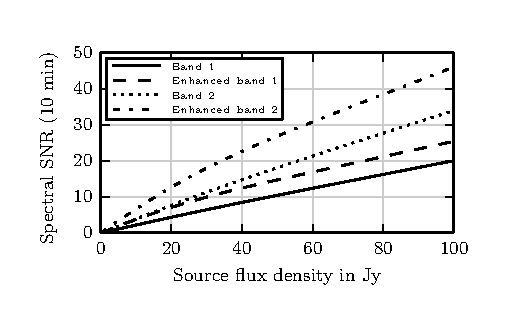
\includegraphics[width=\textwidth]{Figures/f4.eps}
\caption[BETTII Spectral SNR]{%Effects of phase noise and background noise on the spectral $\SNR$. This simulation is computed for BETTII's band 1 parameters and noise estimates, for R=10. We show the results in both the normal science observing mode and the enhanced sensitivity mode. Both simulations are for 200 averaged scans, or 10 minutes on a source. It is important to note that one source can be observed at multiple times during the course of one flight, hence increasing the spectral $\SNR$.
BETTII's spectral sensitivity. Solid: Normal observing mode, band 1; Dashed: Enhanced sensitivity mode, band 1; Dotted: normal observing mode, band 2; Dot-dashed: Enhanced sensitivity mode, band 2. This plot includes the technique of fringe tracking in the science channel for sufficiently bright sources (see Appendix C). As the source flux rises, the effects of the phase noise become larger and the SNR should reach an asymptotical value. However, with fringe tracking, the phase noise itself becomes smaller since one can see fringes in one single or a few consecutive scans, so the co-adding becomes easier. Thanks to the fringe-tracking, there is no regime where the phase noise is expected to be dominant on BETTII, provided that the control system performs according to expectations.}
\label{fig:SpectralSNR}
\end{center}
\end{figure}

Finally, we show the overall sensitivity as a function of point source flux density (Eq.~\ref{eq:noisephth}) for both observing modes and both bands in Figure~\ref{fig:SpectralSNR}. In normal background-limited regime, the sensitivity curves should be straight lines. Here, OPD noise creates a decrease in overall sensitivity as a reduction in coherent power, but also, for brighter targets, from the power lost from the fringe that is converted to white noise (which causes a deviation from straight lines). For very bright targets of 50~Jy or more, it is possible to measure the OPD accurately within each interferogram by tracking the fringes in the science channels themselves (see Appendix~A). For sufficiently large $\SNR$, this process has less error than the assumed $5~\um$ OPD noise coming from the indirect OPD estimation, so the OPD noise decreases for these very large fluxes to become negligible. This is particularly attractive for in-flight testing and calibration.

It is important to note that for sufficiently faint targets, it is impossible to accurately measure the OPD using single scans or co-adds of scans: we rely on the OPD estimator to have sufficient stability to properly co-add scans until the next calibration measurement. This needs to be considered carefully when planning the observation strategy, as long stretches without calibration could lead to a total loss of the OPD information (hence a total loss in scientific data), due to other OPD noise contributors such as thermal drifts that impact the payload on long timescales.
%\subsection{Phase noise mitigation strategies}
%\label{subsec: noisemitigation}

%There are two natural regimes for BETTII's interferograms. First, the high-$\SNR_\mI$ regime exhibits enough SNR that the fringes are visible in one single delay line scan. Second, the low-$\SNR_\mI$ regime does not have enough SNR and requires multiple consecutive interferograms to obtain a usable dataset. 

%In the high $\SNR_\mI$ case, when the source is bright enough to display a detectable fringe pattern in one single scan, then we can self-calibrate each scan with respect to each other by aligning each scan on the center of the fringe packet. We estimate that $\SNR_\mI=2.5$ would allow this. Also, we estimate that our ability to find the center of the fringe with a simple parabolic fit on the envelope has a variance related to $\SNR_\mI$ with the relation $\varPhir = (2\pi)^2 / (N_f\times\samp\times\SNR_\mI^2)$, where $N_f$ is the number of fringes with good $\SNR$ so that $N_f\times\samp$ corresponds to the number of points used to find the fringe center. We do our calculations supposing $N_f=3$ as a minimum. This simple expression merely states that our ability to find the fringe center improves with the square root of the number of samples with good $\SNR$.

%For the low $\SNR$ case, a number of scans are co-added in post-processing, using the post-flight best estimates for the attitude and the ZPD. The phase noise effectively stems from the residual uncertainty in the pointing solution, originating mostly in noise created over timescale~3. One can co-add the smallest amount $M$ of consecutive scans that would average to an overall $\SNR_\mI = 2.5$, effectively binning the 200 interferograms into subsets of $M$ within each track. The overall phase noise residuals (after post-processing) within each subset of scans is what influences the spectral $\SNR$, since a fringe is now visible within each subset, allowing for coherent co-adding of the subsets within a track. This method has the advantage that it relaxes the requirements on the phase estimator, since it can reduce the duration a certain phase noise requirement needs to hold.

%For 200 consecutive interferograms which are binned into subsets of $M$, the phase noise variance is the sum of the phase noise variance within each subset, plus the variance of the error in locating the center of the fringe packet within each subset. The error in locating the fringe center for $\SNR_\mI \sim 2.5$ corresponds to approximately 12\% phase noise for the short band (that is, 12\% rms of the central wavelength $1\over\s_0$). 

%For the short band, one single interferogram has a $\SNR_\mI=1$ for a source flux of 40~Jy. For the long band, it corresponds to about 80~Jy. For example a 20~Jy source in the short band requires $\sim~30$ consecutive scans to reach $\SNR_\mI \sim 2.5$. In order for the estimator not to be the limiting noise factor, it is reasonable to require that its residual noise to be about 12\% phase noise as well. At 3 seconds per scan, this means that the phase estimator needs to be good down to $\sim 5~\um$~rms over 1.5~min, for the short band. This also corresponds to relative attitude knowledge of 0.12~arcsec~rms over the same period. 

%In order to derive an expected spectral sensitivity curve, we suppose that in the short band the phase estimator error within a subset of $M$ scans has a variance that increases linearly with $M$ as $\sigma_M^2 = (2\pi)^2\times (0.12)^2\times (M/30)$, where we supposed a 12\% noise for $M=30$ scans. For sources less than 20~Jy, we suppose a fixed phase noise of 15\%, as fainter sources will benefit from the phase alignment from the brightest sources in the field of view. 

%Once the signal is so bright that a $\SNR_\mI=2.5$ is reached within one scan, the $\SNR_\S$ increases linearly with flux density, since the phase noise becomes quickly negligible.


%\subsection{Calibration}

%Calibration of the transmission profile and instrumental effects will also play an important role and could jeopardize the recovery of the source spectrum. However, it is difficult to measure the overall system's properties from the ground, due to the size of the instrument, the perturbations of the environment and the extremely large far-IR thermal background of ambient-temperature laboratories: interferometry from the ground with far-IR double-Fourier instruments of the size of BETTII is extremely challenging. In-flight calibration observations seem to be the best method of properly understanding the instrument at the system level. 

%Most instrumental effects can be determined by observing bright point sources. This is routinely done in ground-based radio interferometry. However, with BETTII, the sensitivity is such that these sources are rare. In addition it is often difficult to know if a bright far-IR astronomical source is actually a point source when observed at such resolution: this is precisely the problem that BETTII is trying to study. In order to characterize the instrument, we suggest to use bright solar system objects for our bandpass and flux calibrators. Although all the planets are too resolved for BETTII's 8~meter baseline, bright asteroids are not and can have typical fluxes of hundreds of Janskies in the BETTII bands, which provides excellent SNR even in one single delay line scan. 

%\section{Implications for BETTII Observations}
%
%
%
%\subsection{Observing strategies}
%Although it is not possible to achieve better sensitivity than the one imposed by the thermal noise background, there are strategies to keep the phase noise to a minimum over various timescales. With time-domain Fourier Transform spectrometers \citep{Griffiths:2007uu} it is often the case that delay space is scanned rapidly to optimize the integrity of the interferogram and multiple scans are collected to achieve the desired $\SNR$. For the bolometer-type detectors commonly used at infrared wavelengths, and planned for BETTII, short integrations are also favored due to the intrinsic $1/f$ noise \citep{deKorte:2003km}. In our case, however, we expect minimal residual phase noise within each individual scan. This naturally sets two regimes of observations: low $\SNR_\mI$ where the astronomical source is weakly detected or not detected in a single interferogram, and high $\SNR_\mI$ where individual interferograms can be used to estimate ZDP. 
%
%The observations will be divided in tracks of approximately 10 minutes (200 scans of 3 seconds). The scans are composed of 1024 points of 2.5~ms integration time each, in normal observing mode. In the short band, this corresponds to a fringe sampling of $\samp=4$, and in the long band $\samp \sim 7$. We assume that over one track the spatial visibility of the source is unchanged. Observing tracks at multiple baseline angles throughout the night gives us information about the source's spatial distribution. Hence the relevant sensitivity number corresponds to that of one single track of 10 minutes. Of course, this sensitivity can be improved by observing a point source at multiple occurrences during the night.
%
%\subsection{Thermal noise mitigation}
%
%In order to improve significantly the overall sensitivity, it is possible to take advantage of the fact that the delays creating phase noise are well behaved on short timescales. For example, we can decide to reduce the field of view and not cover the full stroke of the delay line, while keeping the scan speed constant. If we shorten the field of view by a factor of 3, then this gives us 3 times the number of interferograms for the same time period, which allows us to pick up interferograms (1-$\sigma$)  in one scan at $\sim~25$~Jy, instead of $\sim~40$~Jy for normal observing. For the first flight, where we will learn more about the perturbations and their exact timescales, it will be possible to tune the scan speed and stroke parameters as the payload is floating.
%
%This mitigation method provides an "enhanced sensitivity" mode and is particularly relevant for fields where we know the emission is localized within a small given region, and not extended over the full $2\times 2$ arcminutes. Note that the region of interest does not need to be centered around the middle of the delay line range in particular.
%
%The prospect of slowing down the scan, rather than reducing the field of view, is more complicated. Indeed, cold delay line is intimately connected to a number of different gains within the detector readout electronics. A good ground calibration is necessary, and it is much harder to change things while in flight, as changing the scan speed without re-tuning the gains could create undesirable effects \citep{Fixsen:1994cs}.
%
%
%
%\subsection{Phase noise mitigations}
%In the high $\SNR_\mI$ case, when the source is bright enough to display a detectable fringe pattern in one single scan, then we can self-calibrate each scan with respect to each other by aligning each scan on the center of the fringe packet. We estimate that $\SNR_\mI=2.5$ would allow this. Also, we estimate that our ability to find the center of the fringe with a simple parabolic fit on the envelope has a variance related to $\SNR_\mI$ with the relation $\varPhir = (2\pi)^2 / (N_f\times\samp\times\SNR_\mI^2)$, where $N_f$ is the number of fringes with good $\SNR$ so that $N_f\times\samp$ corresponds to the number of points used to find the fringe center. We do our calculations supposing $N_f=3$ as a minimum. This simple expression merely states that our ability to find the fringe center improves with the square root of the number of samples with good signal-to-noise ratio..
%
%For the low $\SNR$ case, $M$ scans are co-added blindly in post-processing, using the post-flight best estimates for the attitude and the ZPD. The phase noise effectively corresponds to the error in the pointing solution. One can co-add the smallest amount of consecutive scans that would allow for an overall $\SNR_\mI = 2.5$, effectively binning the 200 interferograms into subsets within each track. The overall phase noise residuals (after post-processing) within each subset of scans is what influences the spectral $\SNR$, since a fringe is now visible within each subset, allowing for coherent co-adding of the subsets within a track. This method has the advantage that it relaxes the requirements on the phase noise estimator, since it can reduce the duration a certain phase noise requirement needs to hold.
%
%For 200 consecutive interferograms which are binned into subsets of $M$, the phase noise variance is the sum of the phase noise variance within each subset, plus the variance of the error in locating the center of the fringe packet within each subset. The error in locating the fringe center for $\SNR_\mI \sim 2.5$ would be approximately equal to the phase noise within each subset for about 12\% phase noise, for the short band. 
%
%For the short band, with normal observing parameters, one single interferogram has a $\SNR_\mI=1$ for a source flux of 40~Jy. For the long band, it corresponds to about 80~Jy. Hence, for example a 20~Jy source in the short band requires $\sim~30$ consecutive scans to reach $\SNR_\mI \sim 2.5$. At 3 second per scan, this means that the phase estimator needs to be good down to $\sim 5~\um$~rms (12\% of the short band central wavelength) over 1.5~min. This also corresponds to an attitude knowledge of 0.12~arcsec~rms. 
%
%In order to derive an expected spectral sensitivity curve, we suppose that in the short band the phase estimator error within a subset of $M$ scans has a variance that increases with $M$ as $\sigma_M^2 = (2\pi)^2\times (0.1)^2\times (M/30)$, where we supposed a 10\% noise for $M=30$ scans. For sources less than 20~Jy, we suppose a fixed phase noise of 15\%, as fainter sources will benefit from the phase alignment from the brightest sources in the field of view. 
%
%Once the signal is so bright that a $\SNR_\mI=2.5$ is reached within one scan, the $\SNR_\S$ increases linearly with flux density, since the phase noise becomes quickly negligible.
%
%
%
%
%\subsection{Faintest detectable targets}
%
%The BETTII 10-minutes sensitivity is estimated in Table \ref{tab:sensitivity}, for $\R=10$ in both bands, assuming the strategies mentioned in the previous paragraphs. The enhanced sensitivity mode shown here assumes a factor of 3 longer integration time per data point. %The complete list of parameters, including efficiencies, is summarized in the appendix in \ref{tab:params}.
%
%
%The 200 scans are co-added assuming that the object's visibility at that baseline orientation is not changing during the integration ($\Vb = $ constant). Those 200 scans correspond to roughly 10 minutes of on-source time. It is important to point out that BETTII would go back to that target in order to observe it at another angle. If that is the case, and the object is a point source for the interferometer, the new 200 scans can be co-added to the previous 200 scans, hence improving significantly the spectral $\SNR$. 
%\section{Calibration}
%\subsection{Overall strategy}
%
%BETTII will need calibrator targets to help understand the properties of the instrument. For BETTII, ground testing at far-IR wavelengths is extremely challenging, so we will have to spend a significant portion of the first flight looking at a bright calibrator targets in order to characterize systematics like the visibility losses, the bandpass filter shape, etc. For this step, we seek a bright calibrator with known spatial distribution and spectrum.
%
%One calibration step which is of paramount importance occurs before we make any science observations. It consists in looking at a bright point source that allows us to locate ZPD for the first time. Although the instrument will be aligned on the ground so that ZPD falls precisely at the middle of the range of the delay line, thermal changes during ascent will certainly change the location of ZPD. By measuring the location of the fringe center on that first delay line scan, it is possible to adjust the external delay line in order to put ZPD in the center of the stroke of the internal delay line. When ZPD is at the center of the scan range, one delay line stroke will go through ZPD for every pixel on the detector.
%
%Between tracks, BETTII will need to look at calibrator targets in order to monitor the variation of instrumental properties with time. To monitor the timescales of changes in phase and tune our pointing and phase estimators, it would be ideal to measure this pointing error as frequently as possible, which is once every scan. These calibrators do not need to be extremely bright - although a minimum number of scans should be required to reach rapid ZPD finding. In addition, we want to limit the slew range from our scientific targets and that calibrator, in order to optimize the time on source and minimize the disturbances to the instrument between science and calibrator targets.
%%\subsection{Errors in the bandpass profile calibration}
%%
%%\textcolor{red}{If we can measure the bandpass profile only to within n\%, how does that impact our estimate of the spectral index? In practice, how do we do this? Do we do some sort of deconvolution, or we simply divide by the bandpass profile?}
%%
%%\textcolor{red}{Ask Lee how this is done most likely, and run simulations.}
%
%%\subsection{Directly measuring the phase}
%
%%It would be convenient to directly measure the group delay of the incoming light, which would provide an absolute measurement of the location of ZPD. We have investigated the feasibility of a near-IR fringe tracking system with simple envelope tracking, as well as dispersed fringe tracking \citep{Rizzo:2012jp}. Although this system would be robust enough to work at low signal-to-noise ratios, it puts considerable requirements on the differential wavefront errors between the two arms, which are hard to control because of the thermal environment at float. Although BETTII will fly this near-IR instrument, its success does not determine the success of the overall mission. [Stephen's comment: Although the technical success of BETTII is not dependent upon the use of such a near-IR instrument, it will include it in order to….
%%(why are we including it?  hope?  future work?  interesting characterization data?)]
%
%
%
%%\subsection{Bandpass profile measurement}
%%% THIS SEEMS ODD HERE... THINKING ABOUT WHERE TO MOVE IT
%%In recovering the scientific signal $\Be\Vb$, one needs to know the bandpass profile, $\eta\Tbp$ (see Fig \ref{fig:Transmission}). While this will be determined to first order from laboratory calibration of the filters, cryostat windows, and detectors, it could be hard to estimate or measure with enough accuracy once the system is fully assembled. 
%%
%%\begin{figure}[ht!]
%%\begin{center}
%%\includegraphics[width=0.49\textwidth]{phasenoise_3.png}
%%\caption[transmission]{Typical transmission profile $\eta\Tbp$ \citep[inspired by the IRAS transmission spectrum,][]{Whelan:2011}. [NEED TO CHANGE THIS WITH CARDIFF DATA]}
%%\label{fig:Transmission}
%%\end{center}
%%\end{figure}
%%
%%To ensure that we obtain a proper end-to-end characterization of our bandpass profile, we plan on including regular calibrator observations during the flight. This calibrator can be used as a bandpass, flux, and phase calibrator at once. Depending on the online stability of the system, these calibrator observations will be more or less frequent. Calibrator choices are discussed in section~\ref{sec:calibrators}.
%
%\subsection{Calibrator selection}
%\label{sec:calibrators}
%
%BETTII requires bright targets of known spectrum and spatial extension in order to achieve good calibration. While some astronomical objects such as YSOs can sometimes provide the required fluxes (more than 60 Jy), their spatial extension is often uncertain - it is precisely the goal of BETTII to determine their spatial extension, or whether these bright sources are composed of multiple, dimmer sources. Previous missions might not have the angular resolution or the detector properties to draw conclusions on the brightest sources (most detectors are optimized for faint targets and hence saturate on the brightest sources, like Spitzer and WISE). 
%
%Among the objects that are very bright within our bands are the planets of the solar system. We have computed the exact distances of the planets during the month of October, 2015, which is approximately the center of our launch window. Only Uranus and Neptune are up in the sky by night, and their respective extensions are 3.7" and 2.3". This is a significant hit on the visibility, and although Uranus is $~1000$ Jy, it is not usable as a reliable calibrator (see Fig. \ref{fig:Visibility}). If they were available in the night sky in 2015, the moons of Jupiter or Saturn would be excellent candidates, provided that the leaking light from the planet does not disturb the observations too much. The moons are point sources for BETTII and there will often be more than one moon within the instrument's field of view, which would help calibrate the drifts within each individual scan, and show how accurately BETTII can measure the relative distance between two sources.
%
%
%
%Since the planets are not useful for next summer, we need to look towards other types of calibrators. Our favorite option is to look at the solar system's asteroids. Asteroids have been used for calibration before, and their thermal emission properties is well understood \citep{1998A&A...338..340M}. Although they are typically one tenth of the flux of Uranus, they are all unresolved so their visibility is unity. In particular, Ceres is a point source about 800 Jy in the short band, which should provide a $\SNR\sim 20$ in one single interferogram scan. In addition, Ceres is an available target during our launch window. Other asteroids, like Vesta and Pallas, are also excellent candidates for calibrating the instrument. Their spectrum has been extensively studied and successfully used as calibrators by other far-IR facilities such as Herschel \citep{Muller:2002je}.



%A mix of other potential targets are discussed in Table~\ref{tab:calibrators}. These targets are all available from our launch site in the night sky throughout the launch window in 2015. All these calibrators are bright enough in the far-IR bands, as well as in the near-IR bands that allow us to track each individual arm and overlap the beams.

%\begin{table*}[ht!]
%
%\begin{center}
%\begin{tabular}{|c|c|c|c|c|c|c|}
%\hline
%\textbf{Name of source} & \textbf{Type} & \multicolumn{3}{|c|}{\textbf{Published Fluxes (Jy)}}& \textbf{Spatial} &\textbf{ Comment} \\
%&  & \textbf{$25\um$} & \textbf{$60 \um$} &\textbf{$100\um$}  &  \textbf{extension?} &\\
%\hline
%
%Betelgeuse & Red giant & 1700 & 299 & 96 & 40 mas &  \\
%\hline
%V* IK Tau & Variable star & 2380 & 332 &103 & ?? &  \\
%\hline
%IC342  & Starburst galaxy & ?? & ?? & ??  & ?? & A. Schulz et al.: The nucleus of the nearby galaxy IC342  \\
%\hline
%EM* LkHA 101  & Star (?) & 364 & 3236 & 4575  & ?? & Looks like a good candidate - A dusty torus around the luminous young star LkHalpha 101 (Tuthill et al.)  \\
%\hline
%HD 36982  & Variable star & 367 & 4800 & 24  & ?? & Promising - see the paper from bob \\
%\hline
%UGCA 39  & Galaxy & 9 & 93 & 227  & ?? &  \\
%\hline
%
%\end{tabular}
%\caption{Calibrators}
%\label{tab:calibrators}
%\end{center}
%\end{table*} 
\section{Conclusion}

%This paper proposes analytical tools to predict the spectral SNR of single-baseline spatio-spectral interferometers, as a function of intensity and phase noise. The phase noise is divided in three major timescales that are relevant to all spatio-spectral instruments. The derived expressions are applied to the case of BETTII, a 8~meter baseline interferometer that pioneers this technology from a balloon platform to study bright star forming regions. We also present methods to mitigate some of the phase noise effects expected in BETTII's data products. 

Spatio-spectral interferometry can enable high resolution spectral imaging of wide fields at
far-IR wavelengths. Implementation of the technique provides some new instrumental
challenges compared to traditional Fourier Transform Spectroscopy, such as the fact that the measured spectrum is a mix of the source's spectral and spatial information.
%complex nature of the source visibility function. The intrinsic interferogram
%has odd symmetry, rather than even symmetry for an FTS, due to the symmetry of the two light
%paths. The source visibility, which can be a complex function, mixes with the spectral
%response to create an interferogram with odd and even symmetry components. The resulting source
%spectrum, which is a mix of spectral and spatial information, can be complex valued function of wavenumber.

%In a double-Fourier system, the zero path difference occurs at a different delay setting for
%each pixel column perpendicular to the baseline vector. As the delay line sweeps the optical path difference
%between the two light paths to create the interferogram for each pixel, it also covers ZPD for
%each pixel. For scientifically interesting field coverages, the delay stroke needed to cover the
%field is equivalent to a spectral resolving power of 100's to 1000's.

In a double-Fourier system, the zero path difference for each detector pixel occurs at a different delay setting of the delay line. The delay stroke needed to cover a scientifically interesting field of view is equivalent to a spectral resolving power of 100's to 1000's for the central pixels.

We present an analysis of the impact of Gaussian intensity and OPD noise on the spectral sensitivity.
Intensity noise, essentially thermal noise from the optics, sky, astrophysical background, and detector, is similar to noise in 
FTS systems with the exception that the longer scan lengths required to cover the spatial
field add noise; this can be mitigated by cutting the interferogram for each pixel  into smaller arrays centered on each source's ZPD to match the desired spectral resolving power, and by apodizing the interferogram to increase sensitivity to the spectral properties of interest. OPD noise is not usually relevant for FTS systems, but is intrinsic to double-Fourier instruments, since the two incoming beams go through long separate paths before combination. For instruments on balloons or in space, the OPD noise is expected to be dominated by disturbances from the instrument and from pointing errors. On average, OPD noise reduces the coherent power in the interferogram, and converts the power lost from the fringe into additional white noise in the spectrum. We argue that there are three relevant noise timescales: the time to take a single data point, the time to collect a complete interferogram, and the time to co-add $M$ interferograms together in a track. The latter corresponds to the timescale that the source spatial visibility function changes significantly, due to the rotation of the baseline angle on the sky.

We derive the spectral sensitivity of double-Fourier instruments to intensity and OPD noise. The expressions in this paper are derived in the general case and can be used to design any instrument that implements this method.

Applied to the case of BETTII, these equations lead to spectral sensitivity estimates of 26 and 14~Jy in its 30-50~$\um$ and 60-110~$\um$ bands, respectively, to achieve a spectral $\SNR=5$ in 10 minutes with $\R=10$ and an assumed OPD noise of $5~\um$ rms.




%BETTII is designed as symmetric double Fourier interferometer to obtain spatial-spectral data over an extended field. The zero path difference in the two arms is swept across the detector array to create a delay spectrum for each detector. 
%
%This paper presents an analytic form for the interferometric signals and their Fourier Transforms, which correspond to the usable scientific data product that BETTII will obtain. The signal-to-noise ratios is greatly influenced by both thermal noise and phase noise components, which both occur in the interferogram domain but have a severe impact in the spectrum. 
%
%We present ways to mitigate both types of noise by strategically controlling the observation and the data reduction process. Using the current estimated parameters of the system, we derive an expected spectral sensivitity of the instrument over 10 minutes, which amounts to 34 Jy in the short band, and 32 Jy in the long band, with a spectral resolution of $\R=10$. Systematic effects could degrade this sensitivity further, and data processing methods like apodization of the interferograms could improve it.
%
%Finally, we identify Ceres and the other bright asteroids as our best candidates for calibrator targets for BETTII's first flight in 2015.
%

%The ability to determine the location of a source on the sky is discussed 



%The optical system is being designed with a high degree of symmetry and a careful selection of structural materials to minimize changes in differential path length along the two arms as the instrument changes temperature from ground-level to flight altitude ($\Delta T$ of 50~K or more). Path length differences can be caused by temperature gradients across the structure; the impact is being minimized by use of carbon-fiber trusses, thermal shielding, and thinned, low heat capacity structures to facilitate rapid cooling.

%The noise power for BETTII at flight altitude a combination of contributions from the sky, the cumulative emissivity of the mirrors outside the dewar, and the dewar window. It is anticipated that the mirror component will dominate in the 30-50 micron band, and the mirrors and sky will contribute significantly in the 60-90 micron band.

%Phase noise in BETTII arises primarily from error in the instantaneous position of the delay line mirrors and uncertainty in the orientation of the baseline vector between the siderostats.  Knowledge of the baseline will be obtained precision gyroscopes and pointing corrections from the tip-tilt mirrors tracking a guide star during observations. The critical measure is one arc-second in truss angle corresponds to 40 microns in optical path difference.



% \acknowledgments

% The material presented in this paper is based upon work supported by NASA Science Mission Directorate through the ROSES/APRA program, with additional support from NASA Goddard Space Flight Center, and NASA GSFC grant NNX11AG92A to the University of Maryland. Work by T. Veach was supported by an appointment to the NASA Postdoctoral Program at GSFC, administered by the Oak Ridge Associated Universities under contract with NASA. We would like to thank the anonymous referee for suggested improvements to the paper.


%\begin{table}[ht!]
%\begin{center}
%\begin{tabular}{|c|c|c|c|}
%\hline 
%\textbf{Parameter} & \textbf{Band 1} & \textbf{Band 2} & \textbf{Comment} \\ 
%\hline 
%Window emissivity & 0.02 & 0.02 & Measured in the lab \\ 
%\hline 
%Telescope emissivity & 0.077 & 0.077 & 10 mirrors at 0.992 reflection\\ 
%\hline 
%Sky radiance & 0.16 W.m$^{-2}$.sr$^{-1}$ & 0.07 W.m$^{-2}$.sr$^{-1}$ & \cite{Harries:1980cva} \\ 
%\hline 
%Window radiance & 0.17 W.m$^{-2}$.sr$^{-1}$ & 0.04 W.m$^{-2}$.sr$^{-1}$ & Blackbody at 240~K \\ 
%\hline 
%Telescope radiance & 0.17 W.m$^{-2}$.sr$^{-1}$ & 0.04 W.m$^{-2}$.sr$^{-1}$ & Blackbody at 240~K \\ 
%\hline 
%Total optical efficiency & 0.3 & 0.3 & Per arm, includes detectors \\ 
%\hline 
%Photon power from the sky & 35 pW & 36 pW & • \\ 
%\hline 
%Photon power from the window & 40 pW &  18 pW & • \\ 
%\hline 
%Photon power from the telescope & 108 pW & 38 pW & • \\ 
%\hline 
%Total absorbed photon NEP & 1.4$\times 10^{-15}$ W.Hz$^{-0.5}$ & 7$\times 10^{-16}$ W.Hz$^{-0.5}$ & From each arm \\ 
%\hline 
%Detector NEP & 3$\times 10^{-16}$ W.Hz$^{-0.5}$ & 3$\times 10^{-16}$ W.Hz$^{-0.5}$ & For each detector \\ 
%\hline 
%Total NEP & 2$\times 10^{-15}$ W.Hz$^{-0.5}$ & 1$\times 10^{-15}$ W.Hz$^{-0.5}$ & For the sum of both arms \\ 
%\hline 
%\end{tabular} 
%\caption{BETTII noise parameters}
%\label{tab:noise}
%\end{center}
%\end{table} 




%\begin{comment}

%\begin{figure}[ht!]
%\begin{center}
%\plotone{f4.eps}
%\caption[Impact of phase noise]{The phase noise affects the signal more for larger wavenumbers. This shows the simulation for band 1 of BETTII. The amount of phase is quantified by its amount in terms of percentage RMS of the wavelength corresponding to the central wavenumber, about 39 microns (256 cm${-1}$) in our case.}
%\label{fig:PhaseNoiseSim}
%\end{center}
%\end{figure}

%\begin{figure}[ht!]
%\begin{center}
%\plotone{f5.eps}
%\caption[exinter]{Example of simulated recovered spectrum of a 40 Jy source over one 10-minute track with $\R=10$, in the presence of  expected thermal noise levels and phase noise of 10\%. The chosen source spectrum follows a simple power law $\S(\s)\propto\s^2$.}
%\label{fig:exinter}
%\end{center}
%\end{figure}

%\begin{figure}[ht!]
%\begin{center}
%\plotone{f6.eps}
%\caption[Phase Noise]{Residual phase noise profile. The phase noise is expressed in percentage of the central wavelength of the short band (\% of 40~$\um$). }
%\label{fig:SpectralSNR}
%\end{center}
%\end{figure}

%\begin{figure}[ht!]
%\begin{center}
%\plotone{f7.eps}
%\caption[Spectral SNR]{Effects of phase noise and background noise on the spectral $\SNR$. This simulation is computed for BETTII's band 1 parameters and noise estimates, for R=10. We show the results in both the normal science observing mode and the enhanced sensitivity mode. Both simulations are for 200 averaged scans, or 10 minutes on a source. It is important to note that one source can be observed at multiple times during the course of one flight, hence increasing the spectral $\SNR$.}
%\label{fig:SpectralSNR}
%\end{center}
%\end{figure}
%\end{comment}
%\begin{figure}[ht!]
%\begin{center}
%\plotone{f8.eps}
%\caption[Visibility]{Effects of source extension with an 8~m baseline interferometer, for band 1. The visibility at the central wavelength is larger than the integrated visibility over the band, especially given that our band is extremely wide.}
%\label{fig:Visibility}
%\end{center}
%\end{figure}

